\documentclass[8pt,landscape]{article}

\usepackage[utf8]{inputenc}
\usepackage{multicol}
\usepackage{parskip}
\usepackage{tabularx}
\usepackage{amsmath}
\usepackage{amssymb}
\usepackage{amsthm}
\usepackage{geometry}
\usepackage{booktabs}
\usepackage{centernot}
\usepackage{hyperref}
\usepackage{eufrak}
\usepackage{graphicx}
\graphicspath{{pics/}}
\geometry{a4paper, left=3mm, right=3mm, top=3mm, bottom=3mm}

\begin{document}
\begin{multicols}{3}

    \section{The Real Number System}

    \subsection{Introduction}

    \subsection{Ordered Field Axioms}


    % \item \textbf{Postulate 1} \emph{Field Axioms} \\
    %     There are functions $+$ and $\cdot$ defined on
    %     $\mathbb{R}^2 := \mathbb{R} \times \mathbb{R}$,
    %     which satisfy the following properties $\forall a, b, c \in \mathbb{R}$

    %     \begin{itemize}
    %         \item \emph{Closure Properties}:
    %             $a + b, \ a \cdot b \in \mathbb{R}$
    %         \item \emph{Associative Properties}:
    %             $a + (b + c) = (a + b) + c$ and
    %             $a \cdot (b \cdot c) = (a \cdot b) \cdot c$
    %         \item \emph{Commutative Properties}:
    %             $a + b = b + a$ and $a \cdot b = b \cdot a$
    %         \item \emph{Distributive Law}:
    %             $a \cdot (b + c) = a \cdot b + a \cdot c$
    %         \item \emph{Existence of Additive Identity}:
    %             There is a unique element $0 \in \mathbb{R}$ such that
    %             $0 + a = a$ for all $a \in \mathbb{R}$
    %         \item \emph{Existence of Multiplicative Identity}:
    %             There is a unique element $1 \in \mathbb{R}$ such that
    %             $1 \neq 0$ and $1 \cdot a = a$ for all $a \in \mathbb{R}$
    %         \item \emph{Existence of Additive Inverses}:
    %             For every $x \in \mathbb{R}$ there is a unique element $-x \in \mathbb{R}$
    %             such that
    %             \[
    %                 x + (-x) = 0
    %             \]
    %         \item \emph{Existence of Multiplicative Inverses}:
    %             For every $x \in \mathbb{R} \setminus \{0\}$ there is a unique element
    %             $x^{-1} \in \mathbb{R}$ such that
    %             \[
    %                 x \cdot (x^{-1}) = 1
    %             \]
    %     \end{itemize}


    % \item \textbf{Postulate 2} \emph{Order Axioms} \\
    %     There is a relation $<$ on $\mathbb{R} \times \mathbb{R}$ that has the following
    %     properties:
    %     \begin{itemize}
    %         \item \emph{Trichotomy Property}:
    %             Given $a, b \in \mathbb{R}$, one and only one of the following statements hold:
    %             \[
    %                 a < b, \ b < a, \ \text{or} \ a = b
    %             \]
    %         \item \emph{Transitive Property}:
    %             For $a, b, c \in \mathbb{R}$
    %             \[
    %                 a < b \ \text{and} \ b < c \implies a < c
    %             \]
    %         \item \emph{Additive Property}:
    %             For $a, b, c \in \mathbb{R}$
    %             \[
    %                 a < b \ \text{and} \ c \in \mathbb{R} \implies a + c < b + c
    %             \]
    %         \item \emph{Multiplicative Properties}:
    %             For $a, b, c \in \mathbb{R}$
    %             \[
    %                 a < b \ \text{and} \ c > 0 \implies ac < bc
    %             \]
    %             and
    %             \[
    %                 a < b \ \text{and} \ c < 0 \implies bc < ac
    %             \]
    %     \end{itemize}

    \textbf{Remark 1.1} \\
    We will assume that the sets $\mathbb{N}$ and $\mathbb{Z}$ satisfy the following
    properties:
    \begin{enumerate}
        \item If $n, m \in \mathbb{Z}$, then $n + m, n - m$ and $mn$ belong to $\mathbb{Z}$
        \item If $n \in \mathbb{Z}$, then $n \in \mathbb{N}$ if and only if $n \geq 1$
        \item There is no $n \in \mathbb{Z}$ that satisfies $0 < n < 1$
    \end{enumerate}

    \textbf{Definition 1.4} \emph{Absolute Value} \\
    The \emph{absolute value} of a number $a \in \mathbb{R}$ is the number
    \[
        |a| :=
        \begin{cases}{}
            a  & a \geq 0 \\
            -a & a < 0 \\
        \end{cases}
    \]

    \textbf{Remark 1.5} The \emph{absolute value} is multiplicative;
    that is, $|ab| = |a||b| \ \forall a, b, \in \mathbb{R}$

    \textbf{Theorem 1.6} \emph{Fundamental Theorem of Absolute Values} \\
    Let $a \in \mathbb{R}$ and $M \geq 0$.
    Then $|a| \leq M \iff -M \leq a \leq M$.

    \textbf{Theorem 1.7} The absolute value satisfies the following three properties:
    \begin{enumerate}
        \item \emph{Positive Definite}:
            For all $a \in \mathbb{R}$, $|a| > 0$ with $|a| = 0$ if and only if $a = 0$.
        \item \emph{Symmetric}:
            For all $a, b, \in \mathbb{R}$, $|a - b| = |b - a|$,
        \item \emph{Triangle Inequalities}:
            For all $a, b \in \mathbb{R}$ \\
            $|a + b| \leq |a| + |b| \ \text{and} \
            \left| |a| - |b| \right| \leq |a - b|$
    \end{enumerate}

    \textbf{Theorem 1.9} Let $x, y, a \in \mathbb{R}$
    \begin{enumerate}
        \item $x < y + \epsilon \ \forall \epsilon > 0 \iff x \leq y$
        \item $x > y - \epsilon \ \forall \epsilon > 0 \iff x \geq y$
        \item $|a| < \epsilon \ \forall \epsilon > 0 \iff a = 0$
    \end{enumerate}


    \subsection{Completeness Axiom}



    \textbf{Definition 1.10} \emph{Upper bounds} \\
    Let $E \subset \mathbb{R}$ be non-empty
    \begin{enumerate}
        \item The set $E$ is said to be \emph{bounded above} if and only if there is an
            $M \in \mathbb{R}$ such that $a \leq M$ for all $a \in E$,
            in which case $M$ is called an \emph{upper bound} of $E$.
        \item A number $s$ is called a \emph{supremum} of the set $E$ if and only if $s$
            is an upper bound of $E$ and $s \leq M$ for all upper bounds $M$ of $E$.
            (In this case we shall say that $E$ has a \emph{finite supremum} $s$ and write
            $s = \sup E$.)
    \end{enumerate}

    \textbf{Remark 1.12}
    If a set has one upper bound, it has infinitely many upper bounds.

    \textbf{Remark 1.13}
    If a set has a supremum, then it has only one supremum.

    \textbf{Theorem} \emph{Approximation Property for Suprema} \\
    If $E$ has a finite supremum and $\epsilon > 0$ is any positive number, then there is a
    point $a \in E$ such that \\
    $\sup E - \epsilon < a \leq \sup E$

    \textbf{Theorem 1.15} \\
    If $E \subset \mathbb{Z}$ has a supremum, then $\sup E \in E$.
    In particular, if the supremum of a set, which contains only integers, exists,
    that supremum must be an integer.

    \textbf{Postulate 3} \emph{Completeness Axiom} \\
    If $E$ is a nonempty subset of $\mathbb{R}$ that is bounded above, then $E$ has a
    finite
    supremum.

    \textbf{Theorem 1.16} \emph{The Archimedean Principle} \\
    Given real numbers $a$ and $b$, with $a > 0$, there is an integer $n \in \mathbb{N}$
    such that $b < na$.

    \textbf{Theorem 1.18} \emph{Density of Rationals} \\
    If $a, b, \in \mathbb{R}$ satisfy $a < b$, then there is a $q \in \mathbb{Q}$
    such that $a < q < b$.

    \textbf{Definition 1.19} \emph{Upper bounds} \\
    Let $E \in \mathbb{R}$ be nonempty
    \begin{enumerate}
        \item The set $E$ is said to be \emph{bounded below} if and only if there is an
            $m \in \mathbb{R}$ such that $a \geq E$, in which case $m$ is called a
            \emph{lower bound} of the set $E$.
        \item A number $t$ is called an \emph{infimum} of the set $E$ if and only if $t$
            is a lower bound of $E$ and $t \geq m$ and write $t = \inf E$.
        \item $E$ is said to be \emph{bounded} if and only if it is bounded both above and
            below.
    \end{enumerate}

    \textbf{Theorem 1.20} \emph{Reflection Principle} \\
    Let $E \in \mathbb{R}$ be nonempty
    \begin{enumerate}
        \item $E$ has a supremum if and only if $-E$ has an infimum, in which case
            $\inf (-E) = -\sup E$.
        \item $E$ has an infimum if and only if $-E$ has a supremum, in which case
            $\sup (-E) = -\inf E$
    \end{enumerate}

    \textbf{Theorem 1.21} \emph{Monotone Property} \\
    Suppose that $A \subseteq B$ are nonempty subsets of $\mathbb{R}$.
    \begin{enumerate}
        \item If $B$ has a supremum, then $\sup A \leq \sup B$.
        \item If $B$ has an infimum, then $\inf A \geq \inf B$.
    \end{enumerate}


    \subsection{Mathematical Induction}



    \textbf{Theorem 1.22} \emph{Well-Ordering Principle} \\
    If $E$ is a nonempty subset of $\mathbb{N}$, then $E$ has a least element
    (i.e.\ $E$ has a finite infimum and $\inf E \in E$).

    \textbf{Theorem 1.23} \\
    Suppose for each $n \in \mathbb{N}$ that $A(n)$ is a proposition which satisfies
    the following two properties:
    \begin{enumerate}
        \item $A(1)$ is true.
        \item For every $n \in \mathbb{N}$ for which $A(n)$ is true, $A(n+1)$ is also true.
    \end{enumerate}
    Then $A(n)$ is true for all $n \in \mathbb{N}$.

    \textbf{Theorem 1.26} \emph{Binomial Formula} \\
    If $a, b, \in \mathbb{R}, n \in \mathbb{N}$ and $0^0$ is interpreted to be $1$, then
    \[
        {(a+b)}^n = \sum_{k=0}^n
        \begin{pmatrix}
            n \\ k
        \end{pmatrix}
        a^{n-k} b^k
    \]


    \subsection{Inverse Functions and Images}



    \textbf{Definition 1.29} \emph{Injection, Surjection, Bijection} \\
    Let $X$ and $Y$ be sets and $f : X \to Y$
    \begin{enumerate}
        \item $f$ is said to be \emph{injective} if and only if
            \[
                x_1, x_2 \in X \ \text{and} \ f(x_1) = f(x_2) \implies x_1 = x_2
            \]
        \item $f$ is said to be \emph{surjective} if and only if
            \[
                \forall y \in Y \ \exists x \in X \backepsilon y = f(x)
            \]

        \item $f$ is called \emph{bijective} if and only if it is both injective
            and surjective
    \end{enumerate}

    \textbf{Theorem 1.30} \\
    Let $X$ and $Y$ be sets and $f : X \to Y$.
    Then the following three statements are equivalent.
    \begin{enumerate}
        \item $f$ has an inverse;
        \item $f$ is injective from $X$ onto $Y$;
        \item There is a function $g : Y \to X$ such that \\
            $g(f(x)) = x \quad \forall x \in X$
            and \\
            $f(g(y)) = y \quad \forall y \in Y$
    \end{enumerate}
    Moreover, for each $f : X \to Y$, there is only one function $g$ that satisfies these.
    It is the inverse function $f^{-1}$.

    \textbf{Remark 1.31} \\
    Let $I$ be an interval and let $f : I \to \mathbb{R}$.
    If the derivative of $f$ is either always positive on $I$, or always negative on $I$,
    then $f$ is injective on $I$.

    \textbf{Definition 1.33} \emph{Image} \\
    Let $X$ and $Y$ be sets and $f : X \to Y$.
    The \emph{image} of a set $E \subseteq X$ under $f$ is the set
    \[
        f(E) := \{ y \in Y : y = f(x) \ \text{for some} \ x \in E \}
    \]
    The \emph{inverse image} of a set $E \subseteq Y$ under $f$ is the set
    \[
        f^{-1}(E) := \{ x \in X : f(x) = y \ \text{for some} \ y \in E \}
    \]

    \textbf{Definition 1.35} \emph{Union, Intersection} \\
    Let $\mathcal{E} = {\{ E_{\alpha} \}}_{\alpha \in A}$ be a collection of sets.
    \begin{enumerate}
        \item The \emph{union} of the collection $\mathcal{E}$ is the set
            \[
                \bigcup_{\alpha \in A} E_\alpha := \{ x : x \in E_\alpha \ \text{for some}
                \ \alpha \in A \}
            \]
        \item The \emph{intersection} of the collection $\mathcal{E}$ is the set
            \[
                \bigcap_{\alpha \in A} E_\alpha := \{ x : x \in E_\alpha \ \text{for all} \
                \alpha \in A \}.
            \]
    \end{enumerate}


    \textbf{Theorem 1.36} \emph{DeMorgan's Laws} \\
    Let $X$ be a set and ${\{ E_\alpha \}}_{\alpha \in A}$ be a collection of subsets of
    $X$.
    If for each $E \subseteq X$ the symbol $E^c$ represents the set $X \setminus E$, then
    ${\left( \bigcup_{\alpha \in A} E_\alpha \right)}^c =
    \bigcap_{\alpha \in A} E_\alpha^c$
    and
    ${\left( \bigcap_{\alpha \in A} E_\alpha \right)}^c =
    \bigcup_{\alpha \in A} E_\alpha ^c$


    \textbf{Theorem 1.37} \\
    Let $X$ and $Y$ be sets and $f : X \to Y$.
    \begin{enumerate}
        \item If ${\{ E_\alpha \}}{\alpha \in A}$ is a collection of subsets of $X$, then \\
            $f \left( \bigcup_{\alpha \in A} E_\alpha \right) =
            \bigcup_{\alpha \in A} f(E_\alpha) \ \text{and} \\
            f \left( \bigcap_{\alpha \in A} E_\alpha \right) \subseteq
            \bigcap_{\alpha \in A} f(E_\alpha)$
        \item If $B$ and $C$ are subsets of $X$, then
            $f(C) \setminus f(B) \subseteq f(C \setminus B)$
        \item If ${\{E_\alpha\}}_{\alpha \in A}$ is a collection of subsets of $Y$, then
            $f^{-1} \left( \bigcup_{\alpha \in A} E_\alpha \right) =
            \bigcup_{\alpha \in A} f^{-1} (E_\alpha) \ \text{and} \ \\
            f^{-1} \left( \bigcap_{\alpha \in A} E_\alpha \right) =
            \bigcap_{\alpha \in A} f^{-1} (E_\alpha)$
        \item If $B$ and $C$ are subsets of $Y$, then
            $f^{-1}(C \setminus B) = f^{-1}(C) \setminus f^{-1}(B)$.
        \item If $E \subseteq f(x)$, then $f(f^{-1}(E)) = E$, but if $E \subseteq X$,
            then $E \subseteq f^{-1}(f(E))$.
    \end{enumerate}



    \subsection{Countable and Uncountable Sets}



    \textbf{Definition 1.38} \emph{Countable \& Uncountable} \\
    Let $E$ be a set.
    \begin{enumerate}
        \item $E$ is said to be \emph{finite} if and only if either $E = \emptyset$
            or there exists an injective function which takes
            $\{ 1, 2, \ldots, n \}$ onto $E$, for some $n \in \mathbb{N}$.
        \item $E$ is said to be \emph{countable} if and only if there exists and injective
            function which takes $\mathbb{N}$ onto $E$.
        \item $E$ is said to be \emph{at most countable} if and only if $E$ is either
            finite or countable.
        \item $E$ is said to be \emph{uncountable} if and only if $E$ is neither finite nor
            countable.
    \end{enumerate}

    \textbf{Remark 1.39} \emph{Cantor's Diagonalisation Argument} \\
    The open interval $(0, 1)$ is uncountable.

    \textbf{Lemma 1.40} \\
    A nonempty set $E$ is at most countable if and only if there is a function $g$ from
    $\mathbb{N}$ onto $E$.

    \textbf{Theorem 1.41} \\
    Suppose $A$ and $B$ are sets.
    \begin{enumerate}
        \item If $A \subseteq B$ and $B$ is at most countable, then $A$ is at most
            countable.
        \item If $A \subseteq B$ and $A$ is uncountable, then $B$ is uncountable.
        \item $\mathbb{R}$ is uncountable.
    \end{enumerate}

    \textbf{Theorem 1.42} \\
    Let $A_1, A_2, \ldots$ be at most countable sets.
    \begin{enumerate}
        \item Then $A_1 \times A_2$ is at most countable.
        \item If
            \[
                E = \bigcup_{j=1}^\infty A_j :=
                \bigcup_{j \in \mathbb{N}} A_j :=
                \{ x : x \in A_j \ \text{for some} \ j \in \mathbb{N} \},
            \]
            then $E$ is at most countable.
    \end{enumerate}

    \textbf{Remark 1.43} \\
    The sets $\mathbb{Z}$ and $\mathbb{Q}$ are countable, but the set of irrationals is
    uncountable.




    \section{Sequences in $\mathbb{R}$}

    \subsection{Limits of Sequences}



    \textbf{Definition 2.1} \emph{Convergence} \\
    A sequence of real numbers $\{ x_n \}$ is set to \emph{converge} to a real number
    $a \in \mathbb{R}$ if and only if for every $\epsilon > 0$ there is an
    $N \in \mathbb{N}$ (which in general depends on $\epsilon$) such that
    \[
        n \geq N \implies |x_n - a| < \epsilon
    \]

    \textbf{Remark 2.4}
    A sequence can have at most one limit.

    \textbf{Definition 2.5} \emph{Subsequence} \\
    By a \emph{subsequence} of a sequence ${\{x_n\}}_{n \in \mathbb{N}}$,
    we shall mean a sequence of the form ${\{x_{n_k}\}}_{k \in \mathbb{N}}$,
    where each $n_k \in \mathbb{N}$ and $n_1 < n_2 < \cdots$.

    \textbf{Remark 2.6} \\
    If ${ \{x_n\} }_{n \in \mathbb{N}}$ converges to $a$ and
    ${ \{x_n_k\} }{k \in \mathbb{N}}$ is any subsequence of
    ${ \{x_n\} }_{n \in \mathbb{N}}$, then $x_n_k$ converges to $a$ as $k \to \infty$.

    \textbf{Definition 2.7} \emph{Bounded Sequences} \\
    Let $\{ x_n \}$ be a sequence of real numbers.
    \begin{enumerate}
        \item The sequence $\{ x_n \}$ is said to be \emph{bounded above} if and only if
            the set $ \{ x_n : n \in \mathbb{N} \}$ is bounded above.
        \item The sequence $\{ x_n \}$ is said to be \emph{bounded below} if and only if
            the set $\{ x_n : n \in \mathbb{N} \}$ is bounded below.
        \item $\{ x_n \}$ is said to be \emph{bounded} if and only if it is bounded both
            above and below.
    \end{enumerate}

    \textbf{Theorem 2.8}
    Every convergent sequence is bounded.


    \subsection{Limit Theorems}



    \textbf{Theorem 2.9} \emph{Squeeze Theorem} \\
    Suppose that $\{x_n\}, \{y_n\}$, and $\{w_n\}$ are real sequences.
    \begin{enumerate}
        \item If $x_n \to a$ and $y_n \to a$ as $n \to \infty$,
            and if there is an $N_0 \in \mathbb{N}$ such that
            \[
                x_n \leq w_n \leq y_n \ \text{for} \ n \geq N_0
            \]
            then $w_n \to a$ as $n \to \infty$.
        \item If $x_n \to 0$ as $n \to \infty$ and $\{y_n\}$ is bounded,
            then $x_n y_n \to 0$ as $n \to \infty$.
    \end{enumerate}

    \textbf{Theorem 2.11} \\
    Let $E \subset \mathbb{R}$.
    If $E$ has a finite supremum (respectively, a finite infimum),
    then there is a sequence $x_n \in E$ such that $x_n \to \sup E$
    (respectively, a sequence $y_n \in E$ such that $y_n \to \inf E$)
    as $n \to \infty$.

    \textbf{Theorem 2.12} \\
    Suppose that $\{x_n\}$ and $\{y_n\}$ are real sequences and that
    $\alpha \in \mathbb{R}$.
    If $\{x_n\}$ and $\{y_n\}$ are convergent, then
    \begin{enumerate}
        \item $\lim_{n \to \infty} (x_n + y_n) =
            \lim_{n \to \infty} x_n + \lim_{n \to \infty} y_n$
        \item $\lim_{n \to \infty} (\alpha x_n) = \alpha \lim_{n \to \infty} x_n$
            and
        \item $\lim_{n \to \infty} (x_n y_n) =
            ( \lim_{n \to \infty} x_n ) (\lim_{n \to \infty} y_n)$ \\
            If, in addition, $y_n \neq 0$ and $\lim_{n \to \infty} y_n \neq 0$, then
        \item $\lim_{n \to \infty} \frac{x_n}{y_n} =
            \frac{\lim_{n \to \infty} x_n}{\lim_{n \to \infty} y_n}$ \\
            (In particular, all these limits exist.)
    \end{enumerate}

    \textbf{Definition 2.14} \emph{Divergence} \\
    Let $\{x_n\}$ be a sequence of real numbers.
    \begin{enumerate}
        \item $\{x_n\}$ is said to \emph{diverge} to $+\infty$ if and only if for each
            $M \in \mathbb{R}$ there is an $N \in \mathbb{N}$ such that \\
            $n \geq N \implies x_n > M$
        \item $\{x_n\}$ is said to \emph{diverge} to $-\infty$ if and only if for each
            $M \in \mathbb{R}$ there is an $N \in \mathbb{N}$ such that \\
            $n \geq N \implies x_n < M$
    \end{enumerate}

    \textbf{Theorem 2.15} \\
    Suppose that $\{x_n\}$ and $\{y_n\}$ are real sequences such that $x_n \to +\infty$
    (respectively, $x_n \to -\infty$) as $n \to \infty$.
    \begin{enumerate}
        \item If $y_n$ is bounded below (respectively, $y_n$ is bounded above), then
            $\lim_{n \to \infty} (x_n + y_n) = +\infty$
        \item If $\alpha > 0$, then
            $\lim_{n \to \infty} (\alpha x_n) = +\infty$
        \item If $y_n > M_0$ for some $M_0 > 0$ and all $n \in \mathbb{N}$, then
            $\lim_{n \to \infty} (x_n y_n) = +\infty$
        \item If $\{y_n\}$ is bounded and $x_n \neq 0$, then
            $\lim_{n \to \infty} \frac{y_n}{x_n} = 0$
    \end{enumerate}

    \textbf{Corollary 2.16} \\
    Let $\{x_n\}$, $\{y_n\}$ be real sequences and $\alpha, x, y$ be extended real numbers.
    If $x_n \to x$ and $y_n \to y$, as $n \to \infty$, then \\
    $\lim_{n \to \infty} (x_n + y_n) = x + y$
    provided that the right side is not of the form $\infty - \infty$, and \\
    $\lim_{n \to \infty} (\alpha x_n) = \alpha x, \quad
    \lim_{n \to \infty} (x_n y_n) = xy$ \\
    provided that none of these products is of the form $0 \cdot \pm \infty$.

    \textbf{Theorem 2.17} \emph{Comparison Theorem} \\
    Suppose that $\{x_n\}$ and $\{y_n\}$ are convergent sequences.
    If there is an $N_0 \in \mathbb{N}$ such that
    $x_n \leq y_n \ \text{for} \ n \geq N_0$
    then
    $\lim_{n \to \infty} x_n \leq \lim_{n \to \infty} y_n$. \\
    In particular, if $x_n \in [a, b]$ converges to some point $c$,
    then $c$ must belong to $[a, b]$.


    \subsection{Bolzano-Weierstrass Theorem}



    \textbf{Definition 2.18} \emph{Increasing, Decreasing} \\
    Let ${\{x_n\}}_{n \in \mathbb{N}}$ be a sequence of real numbers.
    \begin{enumerate}
        \item $\{x_n\}$ is said to be \emph{increasing}
            (respectively, \emph{strictly increasing}) if and only if
            $x_1 \leq x_2 \leq \cdots (\text{respectively}, x_1 < x_2 < \cdots)$.
        \item $\{x_n\}$ is said to be \emph{decreasing}
            (respectively, \emph{strictly decreasing}) if and only if
            $x_1 \geq x_2 \geq \cdots (\text{respectively}, x_1 > x_2 > \cdots)$.
        \item $\{x_n\}$ is said to be \emph{monotone} if and only if it is either
            increasing or decreasing.
    \end{enumerate}

    \textbf{Theorem 2.19} \emph{Monotone Convergence Theorem} \\
    If $\{x_n\}$ is increasing and bounded above, or if $\{x_n\}$ is decreasing and bounded
    below, then $\{x_n\}$ converges to a finite limit.

    \textbf{Definition 2.22} \emph{Nested} \\
    A sequence of sets ${\{I_n\}}_{n \in \mathbb{N}}$ is said to be \emph{nested}
    if and only if
    $I_1 \supseteq I_2 \supseteq \cdots$.

    \textbf{Theorem 2.23} \emph{Nested Interval Property} \\
    If ${\{I_n\}}_{n \in \mathbb{N}}$ is a nested sequence of nonempty closed bounded
    intervals, then $E := \bigcap_{n=1}^\infty I_n$ is nonempty.
    Moreover, if the lengths of these intervals satisfy $|I_n| \to 0$ as $n \to \infty$
    then $E$ is a single point.

    \textbf{Remark 2.24}
    The Nested Interval Property might not hold if ``closed'' is omitted.

    \textbf{Remark 2.25}
    The Nested Interval Property might not hold if ``bounded'' is omitted.

    \textbf{Theorem 2.26} \emph{Bolzano---Weierstrass Theorem} \\
    Every bounded sequence of real numbers has a convergent subsequence.


    \subsection{Cauchy Sequences}



    \textbf{Definition 2.27} \emph{Cauchy} \\
    A sequence of points $x_n \in \mathbb{R}$ is said to be \emph{Cauchy} (in \mathbb{R})
    if and only if for every $\epsilon > 0$ there is an $N \in \mathbb{N}$ such that \\
    $n, m \geq N \implies |x_n - x_m| < \epsilon$

    \textbf{Remark 2.28}
    If $\{x_n\}$ is convergent, then $\{x_n\}$ is Cauchy.

    \textbf{Theorem 2.29} \emph{Cauchy} \\
    Let $\{x_n\}$ be a sequence of real numbers.
    Then $\{x_n\}$ is Cauchy if and only if $\{x_n\}$ converges
    (to some point $a \in \mathbb{R}$).

    \textbf{Remark 2.31}
    A sequence that satisfies $x_{n+1} - x_n \to 0$ is not necessarily Cauchy.


    \subsection{Limits Supremum and Infimum}



    \textbf{Definition 2.32} \emph{Limit Supremum \& Infimum} \\
    Let $\{x_n\}$ be a real sequence.
    Then the \emph{limit supremum} of $\{x_n\}$ is the extended real number \\
    $\limsup_{n \to \infty} x_n := \lim_{n \to \infty} (\sup_{k \geq n} x_k)$ \\
    and the \emph{limit infimum} of $\{x_n\}$ is the extended real number \\
    $\liminf_{n \to \infty} x_n := \lim_{n \to \infty} (\inf_{k \geq n} x_k)$

    \textbf{Theorem 2.35} \\
    Let $\{x_n\}$ be a sequence of real numbers, \\
    $s = \limsup_{n \to \infty} x_n$,
    and $t = \liminf_{n \to \infty} x_n$. \\
    Then there are subsequences ${\{x_n_k\}}_{k \in \mathbb{N}}$ and
    ${\{x_\ell_j\}}_{j \in \mathbb{N}}$ such that
    $x_n_k \to s$ as $k \to \infty$ and $x_\ell_j \to t$ as $j \to \infty$.


    \textbf{Theorem 2.36} \\
    Let $\{x_n\}$ be a real sequence and $x$ be an extended real number.
    Then $x_n \to x$ as $n \to \infty$ if and only if \\
    $\limsup_{n \to \infty} x_n = \liminf_{n \to \infty} x_n = x$.


    \textbf{Theorem 2.37} \\
    Let $\{x_n\}$ be a sequence of real numbers.
    Then $\limsup_{n \to \infty} x_n$ (respectively, $\liminf_{n \to \infty}$) is the
    largest value (respectively, the smallest value) to which some subsequences of
    $\{x_n\}$ converges.
    Namely, if $x_n_k \to x$ as $k \to \infty$, then \\
    $\liminf_{n \to \infty} x_n \leq x \leq \limsup_{n \to \infty} x_n$.

    \textbf{Remark 2.38}
    If $\{x_n\}$ is any sequence of real numbers, then
    $\liminf_{n \to \infty} x_n \leq \limsup_{n \to \infty} x_n$.

    \textbf{Remark 2.39}
    A real sequence $\{x_n\}$ is bounded above if and only if
    $\limsup_{n \to \infty} x_n < \infty$, and is bounded below if and only if
    $\liminf_{n \to \infty} x_n > -\infty$.

    \textbf{Theorem 2.40} \\
    If $x_n \leq y_n$ for $n$ large, then \\
    $\limsup_{n \to \infty} x_n \leq \limsup_{n \to \infty} y_n \ \text{and} \\
    \liminf_{n \to \infty} y_n \leq \liminf_{n \to \infty} y_n$


    \section{Functions on \mathbb{R}}

    \subsection{Two-Sided Limits}



    \textbf{Definition 3.1} \emph{Limits} \\
    Let $a \in \mathbb{R}$, let $I$ be an open interval which contains $a$, and let $f$ be
    a real function defined everywhere on $I$ except possibly at $a$.
    Then $f(x)$ is said to \emph{converge to $L$, as $x$ approaches $a$},
    if and only if for every $\epsilon > 0$ there is a $\delta > 0$
    (which in general depends on $\epsilon, f, I$, and $a$) such that
    \[
        0 < |x - a| < \delta \implies |f(x) - L| < \epsilon
    \]
    In this case we write
    \[
        L = \lim_{x \to a} f(x) \quad \text{or} \quad f(x) \to L \ \text{as} \ x \to a
    \]
    and call $L$ the \emph{limit} of $f(x)$ as $x$ approaches $a$.


    \textbf{Remark 3.4} \\
    Let $a \in \mathbb{R}$, let $I$ be an open interval which contains $a$, and let
    $f$, $g$ be real functions defined everywhere on $I$ except possibly at $a$.
    If $f(x) = g(x)$ for all $x \in I \setminus \{a\}$ and $f(x) \to L$ as
    $x \to a$, then $g(x)$ also has a limit as $x \to a$, and
    \[
        \lim_{x \to a} g(x) = \lim_{x \to a} f(x)
    \]


    \textbf{Theorem 3.6} \emph{Sequential Characterisation of Limits} \\
    Let $a \in \mathbb{R}$, let $I$ be an open interval which contains $a$, and let
    $f$ be a real function defined everywhere on $I$ except possibly at $a$.
    Then
    \[
        L = \lim_{x \to a} f(x)
    \]
    exists if and only if $f(x_n) \to L$ as $n \to \infty$ for every sequence
    $\{x_n\} \in I \setminus \{a\}$ which converges to $a$ as $n \to \infty$.


    \textbf{Theorem 3.8} \\
    Suppose that $a \in \mathbb{R}$, that $I$ is an open interval which contains $a$,
    and that $f$, $g$, are real functions defined everywhere on $I$ except possibly
    at $a$.
    If $f(x)$ and $g(x)$ converge as $x$ approaches $a$, then so do
    $(f + g)(x), (fg)(x), (\alpha f)(x)$, and $(f/g)(x)$
    (when the limit of $g(x)$ is nonzer).
    In fact,
    \begin{align*}{}
        \lim_{x \to a} (f + g)(x) &= \lim_{x \to a} + \lim_{x \to a} g(x) \\
        \lim_{x \to a} (\alpha f)(x) &= \aplha \lim_{x \to a} f(x) \\
        \lim_{x \to a} (fg)(x) &= \lim_{x \to a} \lim_{x \to a} g(x) \\
    \end{align*}
    and (when the limit of $g(x)$ is nonzero)
    \[
        \lim_{x \to a} \left( \frac{f}{g} \right) (x) &=
        \frac{\lim_{x \to a} f(x)}{\lim_{x \to a} g(x)}
    \]


    \textbf{Theorem 3.9} \emph{Squeeze Theorem for Functions} \\
    Suppose that $a \in \mathbb{R}$, that $I$ is an open interval which contains $a$,
    and that $f, g, h$ are real functions defined everywhere on $I$ except possibly at $a$.
    \begin{enumerate}
        \item If $g(x) \leq h(x) \leq f(x) \ \forall x \in I \setminus \{a\}$, and
            \[
                \lim_{x \to a} f(x) = \lim_{x \to a} g(x) = L,
            \]
            then the limit of $h(x)$ exists, as $x \to a$, and
            \[
                \lim_{x \to a} h(x) = L.
            \]
        \item If $|g(x)| \leq M \ \forall x \in I \setminus \{a\}$ and $f(x) \to 0$
            as $x \to a$, then
            \[
                \lim_{x \to a} f(x) g(x) = 0
            \]

    \end{enumerate}


    \textbf{Theorem 3.10} \emph{Comparison Theorem for Functions} \\
    Suppose that $a \in \mathbb{R}$, that $I$ is an open interval which contains $a$,
    and that $f, g$ are real functions defined everywhere on $I$ except possibly at $a$.
    If $f$ and $g$ have a limit as $x$ approaches $a$ and
    $f(x) \leq g(x) \ \forall x \in I \setminus \{a\}$, then
    \[
        \lim_{x \to a} f(x) \leq \lim_{x \to a} g(x)
    \]



    \subsection{One-Sided Limits and Limits at Infinity}



    \textbf{Definition 3.12} \emph{Converge from left \& right} \\
    Let $a \in \mathbb{R}$ and $f$ be a real function.
    \begin{enumerate}
        \item $f(x)$ is said to \emph{converge to $L$ as $x$ approaches $a$ from the right}
            if and only if $f$ is defined on some open interval $I$ with left endpoint $a$
            and for every $\epsilon > 0$ there is a $\delta > 0$
            (which in general depends on $\epsilon, f, I$, and $a$) such that
            \[
                a + \delta \in I \quad \text{and} \quad a < x < a + \delta \implies
                |f(x) - L| < \epsilon
            \]
            in this case we call $L$ the \emph{right-hand limit} of $f$ at $a$,
            and denote it by
            \[
                f(a+) := L =: \lim_{x \to a+} f(x)
            \]
        \item $f(x)$ is said to \emph{converge to $L$ as $x$ approaches $a$ from the left}
            if and only if $f$ is defined on some open interval $I$ with left endpoint $a$
            and for every $\epsilon > 0$ there is a $\delta > 0$
            (which in general depends on $\epsilon, f, I$, and $a$) such that
            \[
                a + \delta \in I \quad \text{and} \quad a < x < a + \delta \implies
                |f(x) - L| < \epsilon
            \]
            in this case we call $L$ the \emph{left-hand limit} of $f$ at $a$,
            and denote it by
            \[
                f(a-) := L =: \lim_{x \to a-} f(x)
            \]
    \end{enumerate}


    \textbf{Theorem 3.14} \\
    Let $f$ be a real function.
    Then the limit
    \[
        \lim_{x \to a} f(x)
    \]
    exists and equals $L$ if and only if
    \[
        L = \lim_{x \to a+} f(x) = \lim_{x \to a-} f(x)
    \]


    \textbf{Definition 3.15} \emph{Convergence} \\
    Let $a, L, \in \mathbb{R}$ and let $f$ be a real function.
    \begin{enumerate}
        \item $f(x)$ is said to \emph{converge} to $L$ as $x \to \infty$ if and only if
            there exists a $c > 0$ such that $(c, \infty) \subset \mathrm{Dom}(f)$
            and given $\epsilon > 0$ there is an $M \in \mathbb{R}$ such that
            $x > M$ implies $|f(x) - L| < \epsilon$, in which case we shall write
            \[
                \lim_{x \to \infty} f(x) = L \quad \text{or} \quad
                f(x) \to L \ \text{as} \ x \to \infty
            \]
            Similarly, $f(x)$ is said to \emph{converge} to $L$ as $x \to -\infty$
            if and only if there exists a $c > 0$ such that
            $(\-infty, -c) \subset \mathrm{Dom}(f)$ and given $\epsilon > 0$ there is
            $M \in \mathbb{R}$ such that $x > M$ implies $|f(x) - L| < \epsilon$,
            in which case we shall write
            \[
                \lim_{x \to \infty} = L \quad \text{or} \quad
                f(x) \to L \ \text{as} \ x \to \infty
            \]
        \item The function $f(x)$ is said to converge to $\infty$ as $x \to a$
            if and only if there is an open interval $I$ containing $a$ such that
            $I \setminus \{a\} \subset \mathrm{Dom}(f)$ and given $M \in \mathrm{R}$
            there is a $\delta > 0$ such that $0 \leq |x - a| < \delta$ implies
            $f(x) < M$, in which case we shall write
            \[
                \lim_{x \to a} f(x) = \infty \quad \text{or} \quad
                f(x) \to \infty \ \text{as} \ x \to a
            \]
            Similarly, $f(x)$ is said to \emph{converge} to $-\infty$ as $x \to a$
            if and only if there is an open interval $I$ containing $a$ such that
            $I \setminus \{a\} \subset \mathrm{Dom}(f)$ and given $M \in \mathbb{R}$
            there is a $\delta > 0$ such that $0 < |x-a| < \delta$ implies $f(x) < M$,
            in which case we shall write
            \[
                \lim_{x \to a} f(x) = -\infty \quad \text{or} \quad
                f(x) \to -\infty \ \text{as} \ x \to a
            \]
    \end{enumerate}

    \textbf{Theorem 3.17} \\
    Let $a$ be an extended real number, and let $I$ be a nondegenerate open interval which
    either contains $a$ or has $a$ as one of its endpoints.
    Suppose further that $f$ is a real function defined on $I$ except possibly at $a$.
    Then
    \[
        \lim_{x \to a; x \in I} f(x)
    \]
    exists and equals $L$ if and only if $f(x_n) \to L$ for all sequences $x_n \in I$
    which satisfy $x_n \neq a$ and $x_n \to a$ as $n \to \infty$.


    \subsection{Continuity}



    \textbf{Definition 3.19} \emph{Continuous} \\
    Let $E$ be a nonempty subset of $\mathbb{R}$ and $f : E \to \mathbb{R}$.
    \begin{enumerate}
        \item $f$ is said to be \emph{continuous at a point $a \in \mathbb{E}$} if and only
            if given $\epsilon > 0$ there is a $\delta > 0$
            (which in general depends on $\epsilon, f$, and $a$) such that
            \[
                |x-a| < \delta \quad \text{and} \quad x \in E \implies
                |f(x) - f(a)| < \epsilon
            \]
        \item $f$ is said to be \emph{continuous on $E$} if and only if $f$ is continuous
            at every $x \in E$.
    \end{enumerate}

    \textbf{Remark 3.20} \\
    Let $I$ be an open interval which contains a point $a$ and $f : I \to \mathbb{R}$.
    Then $f$ is continuous at $a \in I$ if and only if
    \[
        f(a) = \lim_{x \to a} f(x)
    \]

    \textbf{Theorem 3.21} \\
    Suppose that $E$ is a nonempty subset of $\mathbb{R}$, that $a \in E$, and that
    $f : E \to \mathbb{R}$.
    Then the following statements are equivalent:
    \begin{enumerate}
        \item $f$ is continuous at $a \in E$.
        \item If $x_n$ converges to $a$ and $x_n \in E$, then
            $f(x_n) \to f(a)$ as $n \to \infty$.
    \end{enumerate}

    \textbf{Theorem 3.22} \\
    Let $E$ be a nonempty subset of $\mathbb{R}$ and $f, g : E \to \mathbb{R}$.
    If $f, g$ are continuous at a point $a \in E$ (respectively continuous on the set $E$),
    then so are $f+g$, $fg$, and $\alpha f$ (for any $\alpha \in \mathbb{R}$).
    Moreover, $f/g$ is continuous at $a \in E$ when $g(a) \neq 0$
    (respectively, on $E$ when $g(x) \neq 0\ \forall x \in E$).

    \textbf{Definition 3.23} \emph{Composition} \\
    Suppose that $A$ and $B$ are subsets of \mathbb{R}, that $f : A \to \mathbb{R}$
    and $g : B \to \mathbb{R}$.
    If $F(A) \subseteq B$ for every $x \in A$, then the \emph{composition} of $g$ with $f$
    is the function $g \circ f : A \to \mathbb{R}$ defined by
    \[
        (g \circ f) (x) := g(f(x)), \quad x \in A
    \]

    \textbf{Theorem 3.24} \\
    Suppose that $A$ and $B$ are subsets of $\mathbb{R}$, that $f : A \to \mathbb{R}$
    and $g : B \to \mathbb{R}$, and that $f(x) \in B \ \forall x \in A$.
    \begin{enumerate}
        \item If $A := I \setminus \{a\}$, where $I$ is a nondegenerate interval which
            either contains $a$ or has $a$ as one of its endpoints, if
            \[
                L := \lim_{x \to a; x \in I} f(x)
            \]
            exists and belongs to $B$, and if $g$ is continuous and $L \in B$, then
            \[
                \lim_{x \to a; x \in I} (g \circ f) (x) =
                g \left( \lim_{x \to a; x \in I} f(x)\right)
            \]
        \item If $f$ is continuous at $a \in A$ and $g$ is continuous at $f(a) \in B$,
            then $g \circ f$ is continuous at $a \in A$.
    \end{enumerate}

    \textbf{Definition 3.25} \emph{Bounded} \\
    Let $E$ be a nonempty subset of $\mathbb{R}$.
    A function $f : E \to \mathbb{R}$ is said to be \emph{bounded} on E if and only if
    there is an $M \in \mathbb{R}$ such that $|f(x)| \leq M$ for all $x \in E$, in
    which case we shall say that $f$ is \emph{dominated} by $M$ on $E$.

    \textbf{Theorem 3.26} \emph{Extreme Value Theorem} \\
    If $I$ a is closed, bounded interval and $f : I \to \mathbb{R}$ is continuous on $I$,
    then $f$ is bounded on $I$.
    Moreover if
    \[
        M = \sup_{x \in I} f(x) \quad \text{and} \quad m = \inf_{x \in I} f(x)
    \]
    then there exist points $x_m, x_M \in I$ such that
    \[
        f(x_M) = M \quad \text{and} \quad f(x_m) = m
    \]

    \textbf{Remark 3.27}
    The Existence Value Theorem is false if either ``closed'' or ``bounded'' is dropped
    from the hypotheses.

    \textbf{Lemma 3.28} \\
    Suppose that $a < B$ and that $f : [a, b) \to \mathbb{R}$.
    If $f$ is continuous at a point $x_0 \in [a,b)$ and $f(x_0) > 0$,
    then there exist a positive number $\epsilon$ and a point
    $x_1 \in [a, b)$ such that $x_1 > x_0$ and $f(x) > \epsilon \ \forall
    x \in [x_0, x_1]$.

    \textbf{Theorem 3.29} \emph{Intermediate Value Theorem} \\
    Suppose that $a < b$ and that $f : [a, b] \to \mathbb{R}$ is continuous.
    If $y_0$ lies between $f(a)$ and $f(b)$, then there is an $x_0 \in (a, b)$
    such that $f(x_0) = y_0$.

    \textbf{Remark 3.34}
    The composition of two functions $g \circ f$ can be nowhere continuous,
    even though $f$ is discontinuous only on $\mathbb{Q}$ and $g$ is discontinuous
    at only one point.

    \subsection{Uniform Continuity}

    \textbf{Definition 3.35} \emph{Uniform continuity} \\
    Let $E$ be a nonempty subset of $\mathbb{R}$ and $f : E \to \mathbb{R}$.
    Then $f$ is said to be \emph{uniformly continuous} on $E$ if and only if
    for every $\epsilon > 0$ there is a $\delta > 0$ such that
    \[
        |x-a| < \delta \quad \text{and} \quad x, a, \in E \implies |f(x) - f(a)| < \epsilon \quad \forall a \in E
    \]

    \textbf{Lemma 3.38} \\
    Suppose that $E \subseteq \mathbb{R}$ and that $f : E \to \mathbb{R}$
    is uniformly continuous.
    If $x_n \in E$ is Cauchy, the $f(x_n)$ is Cauchy.

    \textbf{Theorem 3.39} \\
    Suppose that $I$ is a closed, bounded interval.
    If $f : I \to \mathbb{R}$ is continuous on $I$, then $f$ is uniformly continuous on
    $I$.

    \textbf{Theorem 3.40} \\
    Suppose that $a < b$ and that $f : (a, b) \to \mathbb{R}$.
    Then $f$ is uniformly continuous on $(a, b)$ if and only if $f$ can be continuously
    extended to $[a, b]$; that is, if and only if there is a continuous function
    $g : [a, b] \to \mathbb{R}$ which satisfies
    \[
        f(x) = g(x), \quad x \in (a, b)
    \]

    \section{Differentiability on \mathbb{R}}

    \subsection{The Derivative}

    \textbf{Definition 4.1} \emph{Differentiable} \\
    A real function $f$ is said to be \emph{differentiable} at a point $a \in \mathbb{R}$
    if and only if $f$ is defined on some open interval $I$ containing $a$ and
    \[
        f'(a) := \lim_{h \to 0} \frac{f(a+h) - f(a)}{h}
    \]
    exists.
    In this case $f'(a)$ is called the \emph{derivative} of $f$ at $a$.

    \textbf{Theorem 4.2} \\
    A real function $f$ is differentiable at some point $a \in \mathbb{R}$ if and only if
    there exist an open interval $I$ and a function $F : I \to \mathbb{R}$ such that
    $a \in I$, $f$ is defined on $I$, $F$ is continuous at $a$, and
    \[
        f(x) = F(x) (x-a) + f(a)
    \]
    holds for all $x \in I$ in which case $F(a) = f'(a)$.

    \textbf{Theorem 4.3} \\
    A real function $f$ is differentiable at $a$ if and only if there is a function
    $T$ of the form $T(x) := m(x)$ such that
    \[
        \lim_{h \to 0} \frac{f(a+h) - f(a) - t(h)}{h} = 0
    \]

    \textbf{Theorem 4.4} \\
    If $f$ is differentiable at $a$, then $f$ is continuous at $a$.

    \textbf{Definition 4.6} \emph{Continuously differentiable} \\
    Let $I$ be a nondegenerate interval.
    \begin{enumerate}
        \item A function $f : I \to \mathbb{R}$ is said to be \emph{differentiable}
            on $I$ if and only if
            \[
                f_i'(a) := \lim_{x \to a; x \in I} \frac{f(x) - f(a)}{x-a}
            \]
            exists and is finite for every $a \in I$.
        \item $f$ is said to be \emph{continuously differentiable} on $I$ if and only if
            $f_I'$ exists and is continuous on $I$.
    \end{enumerate}

    \textbf{Remark 4.9} \\
    $f(x) = |x|$ is differentiable on $[0, 1]$ and on $[-1, 0]$ but not on $[-1, 1]$.

    \subsection{Differentiability Theorems}

    \textbf{Theorem 4.10} \\
    Let $f$ and $g$ be real functions and $\alpha \in \mathbb{R}$.
    If $f$ and $g$ are differentiable at $a$, then $f+g$, $\alpha f$, $f \cdot g$,
    and [when $g(a) \neq 0$] $f/g$ are all differentiable at a.
    In fact,
    \begin{align*}{}
        (f+g)'(a) &= f'(a) + g'(a) \\
        (\alpha f)'(a) &= \alpha f'(a) \\
        (f \cdot g)'(a) &= g(a) g'(a) + f(a) g'(a) \\
        \left( \frac{f}{g}\right)'(a) &= \frac{g(a) f'(a) - f(a) g'(a)}{g^2(a)} \\
    \end{align*}

    \textbf{Theorem 4.11} \emph{Chain Rule} \\
    Let $f$ and $g$ be real functions.
    If $f$ is differentiable at $a$ and $g$ is differentiable at $f(a)$, then
    $g \circ f$ is differentiable at $a$ with
    \[
        (g \circ f)'(a) = g'(f(a))f'(a)
    \]

    \subsection{Mean Value Theorem}

    \textbf{Lemma 4.12} \emph{Rolle's Theorem} \\
    Suppose that $a, b \in \mathbb{R}$ with $a < b$.
    If $f$ is continuous on $[a, b]$, differentiable on $(a, b)$, and if $f(a) = f(b)$,
    then $f'(c) = 0$ for some $c \in (a, b)$.

    \textbf{Remark 4.13} \\
    The continuity hypothesis on Rolle's Theorem cannot be relaxed at even one point
    in $[a, b]$.

    \textbf{Remark 4.14} \\
    The differentiability hypothesis on Rolle's Theorem cannot be relaxed at even one point
    in $[a, b]$.

    \textbf{Theorem 4.15} \\
    Suppose that $a, b, \in \mathbb{R}$ with $a<b$.
    \begin{enumerate}
        \item \emph{Generalised Mean Value Theorem}:
            If $f$, $g$ are continuous on $[a, b]$ and differentiable on $(a, b)$,
            then there is a $c \in (a, b)$ such that
            \[
                g'(c) (f(b) - f(a)) = f'(c) (g(b) - g(a))
            \]

        \item \emph{Mean Value Theorem}:
            If $f$ is continuous on $[a, b]$ and differentiable on $(a, b)$, then there
            is a $c \in (a, b)$ such that
            \[
                f(b) - f(a) = f'(c)(b-A)
            \]

    \end{enumerate}

    \textbf{Definition 4.16} \emph{Increasing, Monotone, Decreasing} \\
    Let $E$ be a nonempty subset of $\mathbb{R}$ and $f : E \to \mathbb{R}$.
    \begin{enumerate}
        \item $f$ is said to be \emph{increasing}
            (respectively, \emph{strictly increasing}) on $E$ if and only if
            $x_1, x_2 \in E$ and $x_1 < x_2 \implies f(x_1) \leq f(x_2)$
            [respectively, $f(x_1) < f(x_2)$].
        \item $f$ is said to be \emph{decreasing}
            (respectively, \emph{strictly decreasing}) on $E$ if and only if
            $x_1, x_2 \in E$ and $x_1 < x_2 \implies f(x_1) \geq f(x_2)$
            [respectively, $f(x_1) > f(x_2)$].
        \item $f$ is said to be \emph{monotone} (respectively, \emph{strictly monotone})
            on $E$ if and only if $f$ is either decreasing or increasing
            (respectively, either strictly decreasing or strictly increasing) on $E$.
    \end{enumerate}

    \textbf{Theorem 4.17} \\
    Suppose that $a, b \in \mathbb{R}$, with $a<b$, that $f$ is continuous on $[a, b]$,
    and that $f$ is differentiable on $(a, b)$.
    \begin{enumerate}
        \item If $f'(x) > 0$ [respectively $f'(x) < 0$] for all $x \in (a, b)$,
            then $f$ is strictly increasing (respectively, strictly decreasing) on
            $[a, b]$.
        \item If $f'(x) = 0$ for all $x \in (a, b)$, then $f$ is constant on $[a, b]$.
        \item If $g$ is continuous on $[a, b]$ and differentiable on $(a, b)$,
            and if $f'(x) = g'(x)$ for all $x \in (a, b)$, then $f-g$ is constant on
            $[a, b]$.
    \end{enumerate}

    \textbf{Theorem 4.18} \\
    Suppose that $f$ is increasing on $[a, b]$
    \begin{enumerate}
        \item If $c \in [a, b)$, then $f(c+)$ exists and $f(c) \leq f(c+)$.
        \item If $c \in (a, b]$, then $f(c-)$ exists and $f(c-) \leq f(c)$.
    \end{enumerate}

    \textbf{Theorem 4.19} \\
    If $f$ is monotone on an interval $I$, then $f$ has at most countable many points
    of discontinuity on $I$.

    \textbf{Theorem 4.21} \emph{Bernoulli's Inequality} \\
    Let $\alpha$ be a positive real number.
    If $0 < \alpha < 1$, then
    ${(1+x)}^\alpha \leq 1 + \alpha x \ \forall x \in [-1, \infty)$,
    and if $\alpha \geq 1$, then
    ${(1+x)}^\alpha \geq 1 + \alpha x \ \forall x \in [-1, \infty)$.

    \textbf{Theorem 4.23} \emph{Intermediate Value Theorem for Derivatives} \\
    Suppose that $f$ is differentiable on $[a, b]$ with $f'(a) \neq f'(b)$.
    If $y_0$ is a real number which lies between $f'(a)$ and $f'(b)$,
    then there is an $x_0 \in (a, b)$ such that $f'(x_0) = y_0$.

    \subsection{Taylor's Theorem and L'Hopital's Rule}

    \textbf{Theorem 4.24} \emph{Taylor's Formula} \\
    Let $n \in \mathbb{N}$ and let $a, b$ be extended real numbers with $a<b$.
    If $f : (a, b) \to \mathbb{R}$, and if $f^{(n+1)}$ exists on $(a, b)$,
    then for each pair of points $x, x_0 \in (a, b)$ there is a number $c$
    between $x$ and $x_0$ such that \\
    $f(x) = f(x_0) + \sum_{k=1}^n \frac{f^{(k)} (x_0)}{k!}{(x-x_0)}^k + \\
    \frac{f^{(n+1)}(c)}{(n+1)!} {(x-x_0)}^{n+1}$

    \textbf{Theorem 4.27} \emph{L'Hopital's Rule} \\
    Let $a$ be an extended real number and $I$ be an open interval which either contains
    $a$ or has $a$ as an endpoint.
    Suppose that $f$ and $g$ are differentiable on $I \setminus \{a\}$ and that
    $g(x) \neq 0 \neq g'(x) \ \forall x \in I \setminus \{a\}$.
    Suppose further that
    \[
        A := \lim_{x \to a; x \in I} f(x) = \lim_{x \to a; x \in I} g(x)
    \]
    is either $0$ or $\infty$.
    If
    \[
        B := \lim_{x \to a; x \in I} \frac{f'(x)}{g'(x)}
    \]
    exists as an extended real number, then
    \[
        \lim_{x \to a; x \in I} \frac{f(x)}{g(x)} =
        \lim_{x \to a; x \in I} \frac{f'(x)}{g'(x)}
    \]

    \subsection{Inverse Function Theorems}

    \textbf{Theorem 4.32} \\
    Let $I$ be a nondegenerate interval and suppose that $f : I \to \mathbb{R}$ is
    injective.
    If $f$ is continuous on $I$, then $J := f(I)$ is an interval, $f$ is strictly
    monotone on $I$, and $f^{-1}$ is continuous and strictly monotone on $J$.

    \textbf{Theorem 4.33} \emph{Inverse Function Theorem} \\
    Let $I$ be an open interval and $f : I \to \mathbb{R}$ be injective and continuous.
    If $b = f(a)$ for some $a \in I$ and if $f'(a)$ exists and is nonzero,
    then $f^{-1}$ is differentiable at $b$ and $(f^{-1})'(b) = \frac{1}{f'(a)}$.

    \section{Riemann Integration}

    \subsection{Introduction}

    \subsection{Step functions and their integrals}

    \textbf{Definition 1} \emph{Step function} \\
    We say that $\phi : \mathbb{R} \to \mathbb{R}$ is a \emph{step function} if there
    exist real numbers $x_0 < x_1 < \cdots < x_n$ (for some $n \in \mathbb{N}$) such that
    \begin{enumerate}
        \item $\phi(x) = 0$ for $x < x_0$ and $x > x_n$
        \item $\phi$ is constant on $(x_{j-1}, x_j) 1 \leq j \leq n$.
    \end{enumerate}

    \textbf{Definition 2} \\
    If $\phi$ is a step function with respect to $\{x_0, x_1, \ldots, x_n\}$
    which takes the value $c_j$ on $(x_{j-1}, x_j)$, then
    \[
        \int \phi := \sum_{j=1}^n c_j (x_j - x_{j-1})
    \]

    \textbf{Proposition 1} \\
    If $\phi$ and $\psi$ are step functions and $\alpha$ and $\beta \in \mathbb{R}$, then
    \[
        \int(\alpha \phi + \beta \psi) = \alpha \int \phi + \beta \int \psi.
    \]

    \subsection{Riemann-integrable functions and their integrals}

    \textbf{Definition 3} \emph{Riemann-integrable} \\
    Let $f : \mathbb{R} \to \mathbb{R}$.
    We say that $f$ is \emph{Riemann-integrable} if for every $\epsilon > 0$
    there exist step functions $\phi$ and $\psi$ such that
    $\phi \leq f \leq \psi$
    and
    $\int \psi - \int \phi < \epsilon$

    \textbf{Theorem 1} \\
    A function $f : \mathbb{R} \to \mathbb{R}$ is Riemann-integrable if and only if \\
    $\sup \{ \int \phi : \phi \ \text{is a step function and} \ \phi \leq f \} = \\
    \inf \{ \int \psi : \psi \ \text{is a step function and} \ \psi \geq f \}$.

    \textbf{Definition 4} \\
    If $f$ is Riemann-integrable we define its integral $\int f$ as the common value \\
    $\int f := \sup \{ \int \phi : \phi \ \text{is a step function and} \ \phi \leq f \} \\
    = \inf \{ \int \psi : \psi \ \text{is a step function and} \psi \geq f \}$.

    \textbf{Theorem 2} \\
    A function $f : \mathbb{R} \to \mathbb{R}$ is Riemann-integrable if and only if there
    exist sequences of step functions $\phi_n$ and $\psi_n$ such that
    $\phi_n \leq f \leq \psi_n \ \forall n, \ \text{and} \
    \int \psi_n - \int \phi_n \to 0$ \\
    If $\phi_n$ and $\psi_n$ are any sequences of step functions satisfying above, then
    $\int \phi_n \to \int f \ \text{and} \ \int \psi_n \to \int f$
    as $n \to \infty$.

    \textbf{Lemma 1} \\
    Let $f : \mathbb{R} \to \mathbb{R}$ be a bounded function with bounded support
    $[a, b]$.
    The following are equivalent:
    \begin{enumerate}
        \item $f$ is Riemann-integrable.
        \item for every $\epsilon > 0$ there exist $a = x_0 < \cdots < x_n = b$ such that,
            if $M_j$ and $m_j$ denote the supremum and infimum values of$f$ on
            $[x_{j-1}, x_j]$ respectively, then
            $\sum_{j-1}^n (M_j - m_j) (x_j - x_{j-1}) < \epsilon$
        \item for every $\epsilon > 0$ there exist $a = x_0 < \cdots < x_n = b$
            such that, with $I_j = (x_{j-1}, x_j)$ for $j \geq 1$,
            $\sum_{j=1}^n \sup_{x, y, \in I_j} |f(x) - f(y)| |I_j| < \epsilon$. \\
            For $f : \mathbb{R} \to \mathbb{R}$ a bounded function with bounded support
            $[a, b]$ and for $a = x_0 < \cdots < x_n = b$,
            let $I_j = (x_{j-1}, x_j), m_j := \inf_{x \in I_j} f(x)$ and
            $M_j := \sup_{x \in I_j} f(x)$. \\
            Define the \emph{lower step function of $f$ with respect to
            $\{x_0, \ldots, x_n\}$} as \\
            $\phi_*(x) = \sum_{j=1}^n m_j \chi_{I_j} + \sum_{j=0}^n \chi_{x_j}$ \\
            and the \emph{upper step function of $f$ with respect to
            $\{x_0, \ldots, x_n\}$} as \\
            $\phi^*(x) = \sum_{j=1}^n M_j \chi_{I_j} + \sum_{j=0}^n \chi_{x_j}$ \\
            Note that $\phi_*$ and $\phi^*$ are step functions, and that
            $\phi_* \leq f \leq \phi^*$.

    \end{enumerate}

    \textbf{Theorem 3} \\
    Suppose $f$ and $g$ are Riemann-integrable and $\alpha$ and $\beta$ are real numbers.
    Then
    \begin{enumerate}
        \item $\alpha f + \beta g$ is Riemann-integrable and \\
            $\int(\alpha f + \beta g) = \alpha \int f + \beta \int g$
        \item If $f \geq 0$ then $\int f \geq 0$; if $f \leq g$ then $\int f \leq \int g$.
        \item $|f|$ is Riemann-integrable and $| \int f| \leq \int |f|$
        \item $\max \{f, g\}$ and $\min \{f, g\}$ are Riemann-integrable.
        \item $fg$ is Riemann-integrable.
    \end{enumerate}

    \textbf{Theorem 4} \\
    If $g : [a, b] \to \mathbb{R}$ is continuous, and $f$ defined by $f(x) = g(x)$
    for $a \leq x \leq b$, $f(x) = 0$ for $x \notin [a, b]$ then $f$ is Riemann-integrable.

    \subsection{Fundamental Theorem of Calculus, and Practical Integration}

    \textbf{Theorem 5} \\
    Let $g : [a, b] \to \mathbb{R}$ be Riemann-integrable.
    For $a \leq x \leq b$ let $G(x) = \int_a^x g$.
    Suppose $g$ is continuous at $x$ for some $x \in [a, b]$.
    [If $x$ is an endpoint, we mean one-sided continuous.]
    Then $G$ is differentiable at $x$ and $G'(x) = g(x)$.
    [If $x$ is an endpoint, we mean one-sided differentiable.]

    \textbf{Theorem 6} \\
    Suppose $f : [a, b] \to \mathbb{R}$ has continuous derivative $f'$ on $[a, b]$.
    Then
    $\int_a^b f' = f(b) - f(a)$.

    \subsection{Integrals and uniform limits of sequences and series of functions}

    \textbf{Theorem 7} \\
    Suppose that $f_n : \mathbb{R} \to \mathbb{R}$ is a sequence if Riemann-integrable
    functions which converges uniformly to a function $f$.
    Suppose that $f_n$ and $f$ are zero outside some common interval $[a, b]$.
    Then $f$ is Riemann-integrable and
    $\int f = \lim_{n \to \infty} \int f_n$.

    \section{Infinite Series of Real Numbers}

    \subsection{Introduction}

    \textbf{Definition 6.1} \emph{Partial sum} \\
    Let $S = \sum_{k=1}^\infty a_k$ be an infinite series with terms $a_k$.
    \begin{enumerate}
        \item For each $n \in \mathbb{N}$, the \emph{partial sum of $S$ of order $n$}
            is defined by \\
            $s_n := \sum_{k=1}^n a_k$
        \item $S$ is said to \emph{converge} if and only if its sequence of partial sums
            $\{s_n\}$ converges to some $s \in \mathbb{R}$ as $n \to \infty$;
            that is, if and only if for every $\epsilon > 0$ there is an
            $N \in \mathbb{N}$ such that $n \geq N \implies |s_n - s| < \epsilon$.
            In this case we shall write \\
            $\sum_{k=1}^\infty a_k = s$ \\
            and call $s$ the \emph{sum}, or \emph{value}, of the series
            $\sum_{k=1}^\infty a_k$
        \item $S$ is said to \emph{diverge} if and only if its sequence of partial sums
            $\{s_n\}$ does not converge as $n \to \infty$.
            When $s_n$ diverges to $+\infty$ as $n \to \infty$, we shall also write \\
            $\sum_{k=1}^\infty a_k = s$
    \end{enumerate}

    \textbf{Theorem 6.5} \emph{Divergence Test} \\
    Let ${\{a_k\}}_{k \in \mathbb{N}}$ be a sequence of real numbers.
    If $a_k$ does not converge to zero, then the series $\sum_{k=1}^\infty a_k$ diverges.

    \textbf{Theorem 6.6} \emph{Telescoping Series} \\
    If $\{a_k\}$ is a convergent real sequence, then
    \[
        \sum_{k=1}^\infty (a_k - a_{k+1}) = a_1 - \lim_{k \to \infty} a_k
    \]

    \textbf{Theorem 6.7} \emph{Geometric Series} \\
    Suppose that $x \in \mathbb{R}$, that $N \in \{ 0, 1, \ldots\}$, and that $0^0$
    is interpreted to be $1$.
    Then the series $\sum_{k=N}^\infty x^k$ converges if and only if $|x| < 1$,
    in which case
    \[
        \sum_{k=N}^\infty x^k = \frac{x^N}{1-x}
    \]
    In particular,
    \[
        \sum_{k=0}^\infty x^k = \frac{1}{1-x}, \quad |x| < 1.
    \]

    \textbf{Theorem 6.8} \emph{The Cauchy Criterion} \\
    Let $\{a_k\}$ be a real sequence.
    Then the infinite series $\sum_{k=1}^\infty a_k$ converges if and only if for every
    $\epsilon > 0$ there is an $N \in \mathbb{N}$ such that
    \[
        m \geq n \geq N \implies \left| \sum_{k=n}^m a_k \right| < \epsilon
    \]

    \textbf{Corollary 6.9} \\
    Let $\{a_k\}$ be a real sequence.
    Then the infinite series $\sum_{k=1}^\infty a_k$ converges if and only if given
    $\epsilon > 0$ there is an $N \in \mathbb{N}$ such that
    \[
        n \geq N \implies \left| \sum_{k=n}^\infty a_k \right| < \epsilon
    \]

    \textbf{Theorem 6.10} \\
    Let $\{a_k\}$ and $\{b_k\}$ be real sequences.
    If $\sum_{k=1}^\infty a_k$ and $\sum_{k=1}^\infty b_k$ are convergent series, then \\
    $\sum_{i=1}^\infty (a_k + b_k) = \sum_{k=1}^\infty a_k + \sum_{k=1}^\infty b_k$ \\
    and \\
    $\sum_{k=1}^\infty (\alpha a_k) = \alpha \sum_{k=1}^\infty a_k$ \\
    for any $\alpha \in \mathbb{R}$.

    \subsection{Series with Nonnegative Terms}

    \textbf{Theorem 6.11} \\
    Suppose that $a_k \geq 0$ for large $k$.
    Then $\sum_{k=1}^\infty a_k$ converges if and only if its sequence of partial sums
    $\{s_n\}$ is bounded; that is, if and only if there exists a finite number $M > 0$
    such that \\
    $\left| \sum_{i=1}^n a_k \right| \leq M \ \forall n \in \mathbb{N}$.

    \textbf{Theorem 6.12} \emph{Integral Test} \\
    Suppose that $f : [1, \infty) \to \mathbb{R}$ is positive and decreasing on
    $[1, \infty)$.
    Then $\sum_{k=1}^\infty f(k)$ converges if and only if $f$ is improperly integrable
    on $[1, \infty)$; that is if and only if
    \[
        \int_1^\infty f(x)\, \mathrm{d}x < \infty
    \]

    \textbf{Corollary 6.13} \emph{$p$-Series Test}
    The series
    \[
        \sum_{i=1}^\infty \frac{1}{k^p}
    \]
    converges if and only if $p > 1$.

    \textbf{Theorem 6.14} \emph{Comparison Test} \\
    Suppose that $0 \leq a_k \leq b_k$ for large $k$.
    \begin{enumerate}
        If $\sum_{k=1}^\infty b_k < \infty$, then $\sum_{k=1}^\infty a_k < \infty$.
        If $\sum_{k=1}^\infty b_k = \infty$, then $\sum_{k=1}^\infty a_k = \infty$.
\end{enumerate}

\textbf{Theorem 6.16} \emph{Limit Comparison Test} \\
Suppose that $a_k \geq 0$, that $b_k > 0$ for large $k$, and that
$L := \lim_{n \to \infty} \frac{a_n}{b_n}$ exists as an extended real number.
\begin{enumerate}
    \item If $0 < L < \infty$, then $\sum_{k=1}^\infty a_k$ converges if and only if
        $\sum_{k=1}^\infty b_k$ converges.
    \item If $L = 0$ and $\sum_{k=1}^\infty b_k$ converges then
        $\sum_{k=1}^\infty a_k$ converges.
    \item If $L = \infty$ and $\sum_{k=1}^\infty b_k$ diverges then
        $\sum_{k=1}^\infty a_k$ diverges.
\end{enumerate}

\subsection{Absolute Convergence}

\textbf{Definition 6.18} \emph{Absolute \& Conditional Convergence} \\
Let $S = \sum_{k=1}^\infty a_k$ be an infinite series.
\begin{enumerate}
    \item $S$ is said to \emph{converge absolutely} if and only if
        $\sum_{k=1}^\infty |a_k| < \infty$
    \item $S$ is said to \emph{converge conditionally} if and only if $S$ converges
        but not absolutely.
\end{enumerate}

\textbf{Remark 6.19} \\
A series $\sum_{k=1}^\infty a_k$ converges absolutely if and only if for every
$\epsilon > 0$ there is an $N \in \mathbb{N}$ such that
\[
    m > n \geq N \implies \sum_{k=n}^m |a_k| < \epsilon
\]

\textbf{Remark 6.20} \\
If $\sum_{k=1}^\infty a_k$ converges absolutely, then $\sum_{k=1}^\infty a_k$
converges, but not conversely.
In particular, there exist conditionally convergent series.


\textbf{Definition 6.21} \emph{Limit supremum} \\
The \emph{limit supremum} of a sequence of real numbers $\{x_k\}$ is defined to be
\[
    \limsup_{k \to \infty} x_k := \lim_{n \to \infty} \left( \sup_{k>n} x_k \right).
\]

\textbf{Remark 6.22} \\
Let $x \in \mathbb{R}$ and $\{x_k\}$ be a real sequence.
\begin{enumerate}
    \item If $\limsup_{k \to \infty} x_k < x$, then $x_k < x$ for large $k$.
    \item If $\limsup_{k \to \infty} x_k > x$, then $x_k > x$ for infinitely many $k$s.
    \item If $x_k \to x$ as $x \to \infty$, then $\limsup_{k \to \infty} x_k = x$.
\end{enumerate}

\textbf{Theorem 6.23} \emph{Root Test} \\
Let $a_k \in \mathbb{R}$ and $r := \limsup_{k \to \infty} |a_k|^{\frac{1}{k}}$.
\begin{enumerate}
    \item If $r < 1$, then $\sum_{k=1}^\infty a_k$ converges absolutely.
    \item If $r > 1$, then $\sum_{k=1}^\infty a_k$ diverges.
\end{enumerate}

\textbf{Theorem 6.24} \emph{Ratio test} \\
Let $a_k \in \mathbb{R}$ with $a_k \neq 0$ for large $k$ and suppose that
\[
    r = \lim_{k \to \infty} \frac{|a_{k+1}|}{|a_k|}
\]
exists as an extended real number.
\begin{enumerate}
    \item If $r < 1$, then $\sum_{k=1}^\infty a_k$ converges absolutely.
    \item If $r > 1$, then $\sum_{k=1}^\infty a_k$ diverges.
\end{enumerate}

\textbf{Remark 6.25}
The Root and Ratio tests are inconclusive when $r = 1$.

\textbf{Definition 6.26} \emph{Rearrangement} \\
A series $\sum_{j=1}^\infty b_j$ is called a \emph{rearrangement} of a series
$\sum_{k=1}^\infty a_k$ if and only if there is an injection
$f : \mathbb{N} \to \mathbb{N}$ such that
\[
    b_{f(k)} = a_k, \quad k \in \mathbb{N}
\]

\textbf{Theorem 6.27} \\
If $\sum_{k=1}^\infty a_k$ converges absolutely and $\sum_{j=1}^\infty b_j$
is any rearrangement of $\sum_{k=1}^\infty a_k$, then $\sum_{j=1}^\infty b_j$
converges and
\[
    \sum_{k=1}^\infty a_k = \sum_{j=1}^\infty b_j
\]

\subsection{Alternating Series}

\textbf{Theorem 6.30} \emph{Abel's Formula} \\
Let ${\{a_k\}}_{k \in \mathbb{N}}$ and ${\{b_k\}}_{k \in \mathbb{N}}$ be real
sequences, and for each pair of integers $n \geq m \geq 1$ set \\
$A_{n, m} := \sum_{k=m}^n a_k$
Then \\
$\sum_{k=m}^n a_k b_k = A_{n, m} b_n - \sum_{k=m}^{n-1} A_{k, m} (b_{k+1} - b_k)$
for all integers $n > m \geq 1$.

\textbf{Theorem 6.31} \emph{Dirichlet's Test} \\
Let $a_k, b_k \in \mathbb{R}$ for $k \in \mathbb{N}$.
If the sequence of partial sums $s_n = \sum_{k=1}^n a_k$ is bounded and
$b_k \to 0$ as $k \to \infty$, then $\sum_{k=1}^\infty a_k b_k$ converges.

\textbf{Corollary 6.32} \emph{Alternating Series Test} \\
If $a_k \to 0$ as $k \to \infty$, then \\
$\sum_{k=1}^\infty {(-1)}^k a_k$ \\
converges.

\section{Infinite Series of Functions}

\subsection{Uniform Convergence of Sequences}

\textbf{Definition 7.1} \emph{Pointwise Convergence} \\
Let $E$ be a nonempty subset of $\mathbb{R}$.
A sequence of functions $f_n : E \to \mathbb{R}$ is said to \emph{converge pointwise}
on $E$ if and only if $f(x) = \lim_{n \to \infty} f_n(x)$ exists for each $x \in E$.

\textbf{Remark 7.2} \\
Let $E$ be a nonempty subset of $\mathbb{R}$.
Then a sequence of functions $f_n$ converges pointwise on $E$, as $n \to \infty$
if and only if for every $\epsilon > 0$ and $x \in E$ there is an $N \in \mathbb{N}$
(which may depend on $x$ as well as $\epsilon$) such that
\[
    n \geq N \implies |f_n(x) - f(x)| < \epsilon
\]

\textbf{Remark 7.3} \\
The pointwise limit of continuous (respectively, differentiable) functions is not
necessarily continuous (respectively, differentiable).

\textbf{Remark 7.4} \\
The pointwise limit of integrable functions is not necessarily integrable.

\textbf{Remark 7.5} \\
There exist differentiable functions $f_n$ and $f$ such that $f_n \to f$ pointwise
on $[0, 1]$ but
\[
    \lim_{n \to \infty} f_n'(x) \neq \left( \lim_{n \to \infty} f_n(x) \right)'
\]
for $x = 1$.

\textbf{Remark 7.6} \\
There exist continuous functions $f_n$ and $f$ such that $f_n \to f$ pointwise on
$[0, 1]$ but
\[
    \lim_{n \to \infty} \int_0^1 f_n(x) \, \mathrm{d}x \neq
    \int_0^1 \left( \lim_{n \to \infty} f_n(x) \right) \, \mathrm{d}x
\]

\textbf{Definition 7.7} \emph{Uniform Convergence} \\
Let $E$ be a nonempty subset of $\mathbb{R}$.
A sequence of function $f_n : E \to \mathbb{R}$ is said to \emph{converge uniformly}
on $E$ to a function $f$ if and only if for every $\epsilon > 0$ there is an
$N \in \mathbb{N}$ such that
\[
    n \geq N \implies |f_n(x) - f(x)| < \epsilon
\]
for all $x \in E$.

\textbf{Theorem 7.9} \\
Let $E$ be a nonempty subset of $\mathbb{R}$ and suppose that $f_n \to f$ uniformly
on $E$, as $n \to \infty$.
If $f_n$ is continuous at some $x_0 \in E$, then $f$ is continuous at $x_0 \in E$.

\textbf{Theorem 7.10} \\
Suppose that $f_n \to f$ uniformly on a closed interval $[a, b]$.
If each $f_n$ is integrable on $[a, b]$, then so is $f$ and
\[
    \lim_{n \to \infty} \int_a^b f_n(x)\, \mathrm{d}x =
    \int_a^b \left( \lim_{n \to \infty} f_n(x)\right)\, \mathrm{d}x
\]
In fact, $\lim_{n \to \infty} \int_a^x f_n(t)\, \mathrm{d}t =
\int_a^x f(t)\, \mathrm{d}t$ uniformly for $x \in [a, b]$.

\textbf{Lemma 7.11} \emph{Uniform Cauchy Criterion} \\
Let $E$ be a nonempty subset of $\mathbb{R}$ and let $f_n : E \to \mathbb{R}$ be
a sequence of functions.
Then $f_n$ converges uniformly on $E$ if and only if for every $\epsilon > 0$
there is an $N \in \mathbb{N}$ such that
\[
    n, m \geq N \implies |f_n(x) - f_m(x)| < \epsilon
\]
for all $x \in E$.

\textbf{Theorem 7.12} \\
Let $(a, b)$ be a bounded interval and suppose that $f_n$ is a sequence of funtions
which converges at some $x_0 \in (a, b)$.
If each $f_n$ is differentiable on $(a, b)$, and $f_n'$ converges uniformly on
$(a, b)$ as $n \to \infty$, the $f_n$ converges uniformly on $(a, b)$ and \\
$\lim_{n \to \infty} f_n'(x) = \left( \lim_{n \to \infty} f_n(x) \right)'$ \\
for each $x \in (a, b)$.

\subsection{Uniform Convergence of Series}

\textbf{Definition 7.13} \emph{Convergence} \\
Let $f_k$ be a sequence of real functions defined on some set $E$ and set
\[
    s_n(k) := \sum_{k=1}^n f_k(x), \quad x \in E, n \in \mathbb{N}
\]
\begin{enumerate}
    \item The series $\sum_{k=1}^n f_k(x)$ is said to \emph{converge pointwise} on $E$
        if and only if the sequence $s_n(x)$ converges pointwise on $E$ as
        $n \to \infty$.
    \item The series $\sum_{k=1}^n f_k(x)$ is said to \emph{converge uniformly} on $E$
        if and only if the sequence $s_n(x)$ converges uniformly on $E$ as
        $n \to \infty$.
    \item The series $\sum_{k=1}^n f_k(x)$ is said to
        \emph{converge absolutely (pointwise)} on $E$ if and only if
        $\sum_{k=1}^n |f_k(x)|$ converges for each $x \in E$.
\end{enumerate}

\textbf{Theorem 7.14} \\
Let $E$ be a nonempty subset of $\mathbb{R}$ and let $\{f_k\}$ be a sequence of real
functions defined on $E$.
\begin{enumerate}
    \item Suppose that $x_0 \in E$ and that each $f_k$ is continuous at $x_0 \in E$.
        If $f = \sum_{k=1}^\infty f_k$ converges uniformly on $E$, then $f$ is
        continuous at $x_0 \in E$.
    \item \emph{Term-by-term integration}.
        Suppose that $E = [a, b]$ and that each $f_k$ is integrable on $[a, b]$.
        If $f = \sum_{k=1}^\infty f_k$ converges uniformly on $[a, b]$, then $f$
        is integrable on $[a, b]$ and
        \[
            \int_a^b \sum_{k=1}^\infty f_k(x)\, \mathrm{d}x =
            \sum_{k=1}^\infty \int_a^b f_k(x)\, \mathrm{d}x.
        \]
    \item \emph{Term-by-term differentiation}.
        Suppose that $E$ is a bounded, open interval and that each $f_k$ is
        differentiable on $E$.
        If $\sum_{k=1}^\infty f_k$ converges at some $x_0 \in E$,
        and $\sum_{k=1}^\ingty f_k'$ converges uniformly on $E$,
        then $f := \sum_{k=1}^\infty f_k$ converges uniformly on $E$,
        $f$ is differentiable on $E$, and
        \[
            \left( \sum_{k=1}^\infty f_k(x) \right)' =
            \sum_{k=1}^\infty f_k'(x)
        \]
        for $x \in E$.
\end{enumerate}

\textbf{Theorem 7.15} \emph{Weierstrass $M$-Test} \\
Let $E$ be a nonempty subset of $\mathbb{R}$,
let $f_k : E \to \mathbb{R}, k \in \mathbb{N}$,
and suppose that $M_k \geq 0$ satisfies $\sum_{k=1}^\infty M_k < \infty$.
If $|f_k(x)| \leq M_k$ for $k \in \mathbb{N}$ and $x \in E$, then
$\sum_{k=1}^\infty f_k$ converges absolutely and uniformly on $E$.

% \textbf{Theorem 7.16*} \emph{Dirichlet's Test for Uniform Convergence} \\
% Let $E$ be a nonempty subset of $\mathbb{R}$ and suppose that
% $f_k, g_k : E \to \mathbb{R}, k \in \mathbb{N}$.
% If
% \[
%     \left| \sum_{k=1}^n f_k(x) \right| \leq M < \infty
% \]
% for $n \in \mathbb{N}$ and $x \in E$, and if $g_k \downarrow 0$ uniformly on $E$
% as $k \to \infty$, then $\sum_{k=1}^\infty f_k g_k$ converges uniformly on $E$.

\subsection{Power Series}

\textbf{Definition} \emph{Power Series} \\
Let $(a_n)$ be a sequence of real numbers, and $c \in \mathbb{R}$.
A \emph{power series} is a series of the form \\
$\sum_{n=1}^\infty a_n{(x-c)}^n$ \\
With $a_n$ being the \emph{coefficients} and $c$ its centre.

\textbf{Definition} \emph{Radius of Convergence} \\
The \emph{radius of convergence} $R$ of the power series \\
$\sum_{n=1}^\infty a_n{(x-c)}^n$ \\
is defined by \\
$R = \sup \{ r \geq 0 : (a_n r^n) \ \text{is bounded} \}$ \\
unless $(a_n r^n)$ is bounded for all $r \geq 0$, in which case we declare
$R = \infty$.

\textbf{Theorem 1} \\
Suppose the radius of convergence $R$ satisfies $0 < R < \infty$.
If $|x - c| < R$, the power series converges absolutely.
If $|x - c| > R$, the power series diverges.

\textbf{Theorem 2} \\
Assume that $R > 0$.
Suppose that $0 < r < R$.
Then the series converges uniformly and absolutely on $|x-c| \leq r$ to a continuous
function $f$.
Hence \\
$f(x) = \sum_{n=0}^\infty a_n{(x-c)}^n$ \\
defines a continuous function $f : (c - R, c + R) \to \mathbb{R}$.

\textbf{Lemma} \\
The two power series $\sum_{n=1}^\infty a_n {(x-c)}^n$ and
$\sum_{n=1}^\infty n a_n {(x-c)}^{n-1}$ have the same radius of convergence.

\textbf{Theorem 3} \\
Suppose the radius of convergence of the power series is $R$.
Then the function \\
$f(x) = \sum_{n=0}^\infty a_n {(x-c)}^n$ \\
is infinitely differentiable on $|x-c| < R$, and for such $x$, \\
$f'(x) = \sum_{n=0}^\infty n a_n {(x-c)}^{n-1}$ \\
and the series converges absolutely, and also uniformly on $[c-r, c+r] \ \forall r<R$.
Moreover $a_n = \frac{f^{(n)}(c)}{n!}$

\section{Metric Spaces}

\subsection{Introduction}

\textbf{Definition 10.1} \emph{Metric Space} \\
A \emph{metric space} is a set $X$ together with a function
$\rho : X \times X \to \mathbb{R}$ (called the \emph{metric} of $\rho$) which
satisfies the following properties for all $x, y, z \in X$:
\begin{align*}{}
    \text{Positive Definite} \quad & \rho(x, y) \geq 0 \ \text{with} \ \rho(x, y) = 0
    \iff x = y \\
    \text{Symmetric} \quad & \rho(x, y) = \rho(y, x) \\
    \text{Triangle Inequality} \quad & \rho(x, y) \leq \rho(x, z) + \rho(z, y) \\
\end{align*}

\textbf{Definition 10.7} \emph{Ball} \\
Let $a \in X$ and $r > 0$.
Then \emph{open ball} (in $X$) with \emph{centre} $a$ and \emph{radius} $r$ is the set \\
$B_r(a) := \{ x \in X : \rho(x, a) < r \}$ \\
and the \emph{closed ball} (in $X$) with \emph{centre} $a$ and \emph{radius} $r$ is
the set \\
$\{ x \in X : \rho (x, a) \leq r \}$

\textbf{Definition 10.8} \emph{Open \& Closed}
\begin{enumerate}
    \item A set $V \subseteq X$ is said to be \emph{open} if and only if
        for every $x \in V$ there is an $\epsilon > 0$ such that the open ball
        $B_\epsilon (x)$ is contained in $V$.
    \item A set $E \subseteq X$ is set to be \emph{closed} if and only if
        $E^c := X \setminus E$ is open.
\end{enumerate}

\textbf{Remark 10.9}
Every open ball is open, and every closed ball is closed.

\textbf{Remark 10.10}
If $a \in X$, then $X \setminus \{a\}$ is open, and $\{a\}$ is closed.

\textbf{Remark (10.11)}
In an arbitrary metric space, the empty set $\emptyset$ and the whole space $X$
are both open and closed.

\textbf{Definition 10.13} \emph{Convergence, Cauchy, \& Boundedness} \\
Let $\{x_n\}$ be a sequence in $X$.
\begin{enumerate}
    \item $\{x_n\}$ \emph{converges} (in $X$) if there is a point $a \in X$
        (called the \emph{limit} of $x_n$) such that for every $\epsilon > 0$
        there is an $N \in \mathbb{N}$ such that \\
        $n \geq N \implies \rho(x_n, a) < \epsilon$.
    \item $\{x_n\}$ is \emph{Cauchy} if for every $\epsilon > 0$ there is an
        $N \in \mathbb{N}$ such that \\
        $n, m \geq N \implies \rho(x_n, x_m) < \epsilon$.
    \item $\{x_n\}$ is \emph{bounded} if there is an $M > 0$ and a $b \in X$ such that
        $\rho (x_n, b) \leq M$ for all $n \in \mathbb{N}$.
\end{enumerate}

\textbf{Theorem 10.14} \\
Let $X$ be a metric space.
\begin{enumerate}
    \item A sequence $X$ can have at most one limit.
    \item If $x_n \in X$ converges to $a$ and $\{x_{n_k}\}$ is any subsequence of
        $\{x_n\}$, then $x_{n_k}$ converges to $a$ as $k \to \infty$.
    \item Every convergent sequence $X$ is bounded.
    \item Every convergent sequence in $X$ is Cauchy.
\end{enumerate}

\textbf{Remark 10.15} \\
Let $x_n \in X$.
Then $x_n \to a$ as $n \to \infty$ if and only if for every open set $V$ which
contains $a$, there is an $N \in \mathbb{N}$ such that $n \geq N \implies x_n \in V$.

\textbf{Theorem 10.16} \\
Let $E \subseteq X$.
Then $E$ is closed if and only if the limit of every convergent sequence $x_k \in E$
satisfies \\
$\lim_{k \to \infty} x_k \in E$.

\textbf{Remark 10.17}
The discrete space contains bounded sequence which have no convergent subsequences.

\textbf{Remark 10.18}
The metric space $X = \mathbb{Q}$ contains Cauchy sequences which do not converge.

\textbf{Definition 10.19} \emph{Completeness} \\
A metric space $X$ is said to be \emph{complete} if and only if every Cauchy sequence
$x_n \in X$ converges to some point in $X$.

\textbf{Remark 10.20} \\
By \emph{10.19}, a complete metric space $X$ satisfies two properties:
\begin{enumerate}
    \item Every Cauchy sequence in $X$ converges;
    \item the limit of every Cauchy sequence in $X$ stay in $X$.
\end{enumerate}

\textbf{Theorem 10.21} \\
Let $X$ be a complete metric space $E$ be a subset of $X$.
Then $E$ (as a subspace) is complete if and only if $E$ as a (subset) is closed.

\subsection{Limits of Functions}

\textbf{Definition 10.22} \emph{Cluster Point} \\
A point $a \in X$ is said to be a \emph{cluster point} (of $X$) if and only if
$B_\delta (a)$ contains infinitely many points for each $\delta > 0$.

\textbf{Definition 10.25} \emph{Converge} \\
Let $a$ be a cluster point of $X$ and $f : X \setminus \{a\} \to Y$.
Then $f(x)$ is said to \emph{converge to $L$, as $x$ approaches $a$},
if and only if for every $\epsilon > 0$ there is a $\delta > 0$ such that
\[
    0 < \rho (x, a) < \delta \implies \tau (f(x), L) < \epsilon.
\]
In this case we write $f(x) \to L$ as $x \to a$, or
\[
    L = \lim_{x \to a} f(x),
\]
and call $L$ the \emph{limit} of $f(x)$ as $x$ approaches $a$.

\textbf{Theorem 10.26} \\
Let $a$ be a cluster point of $X$ and $f, g : X \setminus \{a\} \to Y$.
\begin{enumerate}
    \item If $f(x) = g(x) \ \forall x \in X \setminus \{a\}$ and $f(x)$ has a limit
        as $x \to a$, then $g(x)$ also has a limit as $x \to a$, and
        \[
            \lim_{x \to a} g(x) = \lim_{x \to a} f(x).
        \]
    \item \emph{Sequential characterisation of limits}.
        The limit
        \[
            L := \lim_{x \to a} f(x)
        \]
        exists if and only if $f(x_n) \to L$ as $n \to \infty$ for every sequence
        $x_n \in X \setminus \{a\}$ which converges to $a$ as $n \to \infty$.
    \item Suppose that $Y = \mathbb{R}^n$.
        If $f(x)$ and $g(x)$ have a limit as $x$ approaches $a$, then so do
        $(f+g)(x), (f \cdot g)(x), (\alpha f)(x)$, and $(f/g)(x)$
        [when $Y = \mathbb{R}$ and the limit of $g(x)$ is nonzero].
        In fact,
        \begin{align*}
            \lim_{x \to a} (f+g)(x) &= \lim_{x \to a} f(x) + \lim_{x \to a} g(x), \\
            \lim_{x \to a} (\alpha f) (x) &= \alpha \lim_{x \to a} f(x), \\
            \lim_{x \to a} (f \cdot g) (x) &= \lim_{x \to a} f(x) \cdot \lim_{x \to a} g(x)
        \end{align*}
        and [when $Y = \mathbb{R}$ and the limit of $g(x)$ is nonzero]
        \[
            \lim_{x \to a} \left( \frac{f}{g} \right) (x) =
            \frac{\lim_{x \to a} f(x)}{\lim_{x \to a} g(x)}
        \]
    \item \emph{Squeeze Theorem for Functions}.
        Suppose that $Y = \mathbb{R}$.
        If $h : X \setminus \{a\} \to \mathbb{R}$ satisfies
        $g(x) \leq h(x) \leq f(x) \ \forall x \in X \setminus \{a\}$, and
        \[
            \lim_{x \to a} f(x) = \lim_{x \to a} g(x) = L
        \]
        then the limit of $h$ exists, as $x \to a$, and
        \[
            \lim_{x \to a} h(x) = L
        \]
    \item \emph{Comparison Theorem for Functions}.
        Suppose that $Y = \mathbb{R}$.
        If $f(x) \leq g(x) \ \forall X \setminus \{a\}$, and if $f$ and $g$ have
        a limit as $x$ approaches $a$, then
        \[
            \lim_{x \to a} f(x) \leq \lim_{x \to a} g(x)
        \]

\end{enumerate}

\textbf{Definition 10.27} \emph{Continuity} \\
Let $E$ be a nonempty subset of $X$ and $f : E \to Y$.
\begin{enumerate}
    \item $f$ is said to be \emph{continuous at a point} $a \in E$ if and only if
        given $\epsilon > 0$ there is a $\delta > 0$ such that
        \[
            \rho (x, a) < \delta \ \text{and} \ \x \in E \implies
            \tau (f(x), f(a)) < \epsilon.
        \]
    \item $f$ is said to be \emph{continuous on $E$} if and only if $f$ is
        continuous at every $x \in E$.
\end{enumerate}

\textbf{Theorem 10.28} \\
Let $E$ be a nonempty subset of $X$ and $f, g : E \to Y$.
\begin{enumerate}
    \item $f$ is continuous at $a \in E$ if and only if $f(x_n) \to f(a)$,
        as $n \to \infty$, for all sequences $x_n \in E$ which converge to $a$.
    \item Suppose that $Y = \mathbb{R}^n$.
        If $f, g$ are continuous at a point $a \in E$ (respectively continuous on
        a set $E$), then so are $f+g, f \cdot g$, and $\alpha f$
        (for any $\alpha \in \mathbb{R}$).
        Moreover, in the case $Y = \mathbb{R}$, $f/g$ is continuous at $a \in E$
        when $g(a) \neq 0$ [respectively, on $E$ when $g(x) \neq 0,
        \ \forall x \in E$].
\end{enumerate}

\textbf{Theorem 10.29} \\
Suppose that $X, Y$, and $Z$ are metric space and that $a$ is a cluster point of $X$.
Suppose further that $f : X \to Y$ and $g : f(X) \to Z$.
If $f(x) \to L$ as a $x \to a$ and $g$ is continuous at L, then
\[
    \lim_{x \to a} (g \circ f) (x) = g \left( \lim_{x \to a} f(x) \right).
\]

\textbf{Definition 10.30} \emph{Bolzano-Weierstrass Property} \\
$X$ is said to satisfy the \emph{Bolzano-Weierstrass Property} if and only if every
bounded sequence $x_n \in X$ has a convergent subsequence.

\subsection{Interior, Closure, and Boundary}

\textbf{Theorem 10.31} \\
Let $X$ be a metric space.
\begin{enumerate}
    \item If ${\{V_\alpha\}}_{\alpha \in A}$ is any collection of open sets in $X$,
        then $\bigcup_{\alpha \in A} V_\alpha$
        is open.
    \item If $\{V_k : k = 1, 2, \ldots, n\}$ is a finite collection of open sets in
        $X$, then
            $\bigcap_{k=1}^n V_k := \bigcap_{k \in \{1, 2, \ldots, n\}} V_k$
        is open.
    \item If ${\{E_\alpha\}}_{\alpha \in A}$ is any collection of closed sets in $X$,
        then $\bigcap_{\alpha \in A} E_\alpha$ is closed.
    \item If $\{E_k : k = 1, 2, \ldots, n\}$ is a finite collection of closed sets in
        $X$, then
            $\bigcup_{k=1}^n E_k := \bigcup_{k \in \{1, 2, \ldots, n\}} E_k$
        is closed.
    \item If $V$ is open in $X$ and $E$ is closed in $X$, then $V \setminus E$
        is open and $E \setminus V$ is closed.
\end{enumerate}


\textbf{Remark 10.32} \\
Statements 2 and 4 of \emph{Theorem 10.31} are false if arbitrary collections are used
in place of finite collections.


\textbf{Definition 10.33} \emph{Interior \& Closure} \\
Let $E$ be a subset of a metric space $X$.
\begin{enumerate}
    \item The \emph{interior} of $E$ is the set
        \[
            E^O := \bigcup \{ V : V \subseteq E \
            \text{and} \ V \ \text{is open in} \ X\}.
        \]
    \item The \emph{closure} of $E$ is the set
        \[
            \overline{E} := \bigcap \{ B : B \supseteq E \
            \text{and} \ B \ \text{is closed in} \ X\}.
        \]
\end{enumerate}

\textbf{Theorem 10.34} \\
Let $E \subseteq X$.
Then
\begin{enumerate}
    \item $E^O \subseteq E \subseteq \overline{E}$,
    \item if $V$ is open and $V \subseteq E$, then $V \subseteq E^0$, and
    \item if $C$ is closed and $C \supseteq E$, then $C \supseteq \overline{E}$.
\end{enumerate}


\textbf{Definition 10.37} \emph{Boundary} \\
Let $E \subseteq X$.
The \emph{boundary} of $E$ is the set
\[
    \partial E := \{x \in X : \forall r > 0, \ B_r(x) \cap E \neq \emptyset \
    \text{and} \ B_r(x) \cup E^c \neq \emptyset \}.
\]
[We refer to the last two conditions in the definition of $\partial E$ by saying
$B_r(x)$ \emph{intersects} $E$ and $E^c$.]


\textbf{Theorem 10.39} \\
Let $E \subseteq X$.
Then
\[
    \partial E = \overline{E} \setminus E^0.
\]


\textbf{Theorem 10.40} \\
Let $A, B \subseteq X$.
Then
\begin{enumerate}
    \item ${(A \cup B)}^O \supseteq A^O \cup B^O$, \quad
        ${(A \cap B)}^O = A^O \cap B^O$,
    \item $\overline{A \cup B} = \overline{A} \cup \overline{B}, \quad
        \overline{A \cap B} \subseteq \overline{A} \cap \overline{B}$,
    \item $\partial (A \cup B) \subseteq \partial A \cup \partial B$, \quad and \quad
        $\partial (A \cap B) \subseteq (A \cap \partial B) \cup (B \cap \partial A) \cup
        (\partial A \cap \partial B)$.
\end{enumerate}

\subsection{Compact Sets}

\textbf{Definition 10.41} \emph{Covering} \\
Let $\mathcal{V} = {\{V_\alpha\}}_{\alpha \in A}$ be a collection of subsets of a
metric space $X$ and suppose that $E$ is a subset of $X$.
\begin{enumerate}
    \item $\mathcal{V}$ is said to \emph{cover} $E$ if and only if
        \[
            E \subseteq \bigcup_{\alpha \in A} V_\alpha.
        \]

    \item $\mathcal{V}$ is said to be an \emph{open covering} of $E$ if and only if
        $\mathcal{V}$ covers $E$ and each $V_\alpha$ is open.
    \item Let $\mathcal{V}$ be a covering of $E$.
        $\mathcal{V}$ is said to have a \emph{finite} (respectively \emph{countable})
        \emph{subcovering} if and only if there is a finite (respectively, countable)
        subset $A_0$ of $A$ such that ${\{V_\alpha\}}_{\alpha \in A_0}$ covers $E$.
\end{enumerate}


\textbf{Definition 10.42} \emph{Compact} \\
A subset $H$ of a metric space $X$ is said to be \emph{compact} if and only if every
open covering of $H$ has a finite subcover.


\textbf{Remark 10.43}
The empty set and all finite subsets of a metric space are compact.


\textbf{Remark 10.44}
A compact set is always closed.


\textbf{Remark 10.45}
A closed subset of a compact set is compact.


\textbf{Theorem 10.46} \\
Let $H$ be a subset of a metric space $X$.
If $H$ is compact, then $H$ is closed and bounded.


\textbf{Remark 10.47}
The converse of \emph{Theorem 10.46} is false for arbitrary metric spaces


\textbf{Definition 10.48} \emph{Separable} \\
A metric space $X$ is said to be \emph{separable} if and only if it contains a
countable dense subset
(i.e.\ if and only if there is a countable subset $Z$ of $X$ such that for every
point $a \in X$ there is a sequence $x_k \in Z$ such that $x_k \to a$ as
$k \to \infty$).


\textbf{Theorem 10.49} \emph{Lindel\"of} \\
Let $E$ be a subset of a separable metric space $X$.
If ${\{V_\alpha\}}_{\alpha \in A}$ is a collection of open sets and
$E \subseteq \bigcup_{\alpha \in A} V_\alpha$, then there is a countable subset
$\{ \alpha_1, \alpha_2, \ldots \}$ of $A$ such that
\[
    E \subseteq \bigcup_{k=1}^\infty V_{\alpha_k}
\]

\textbf{Theorem 10.50} \emph{Heine-Borel} \\
Let $X$ be a separable metric space which satisfies the
\emph{Bolzano-Weierstrass Property}, and $H$ be a subset of $X$.
Then $H$ is compact if and only if it is closed and bounded.

\textbf{Definition 10.51} \emph{Uniform Continuity} \\
Let $X$ be a metric space, $E$ be a nonempty subset of $X$, and $f : E \to Y$.
Then $f$ is said to be \emph{uniformly continuous} on $E$ if and only if given
$\epsilon > 0$ there is a $\delta > 0$ such that
\[
    \rho (x, a) < \delta \ \text{and} \ x, a \in E \implies
    \tau (f(x), f(a)) < \epsilon.
\]

\textbf{Theorem 10.52} \\
Suppose that $E$ is a compact subset of $X$ and that $f : X \to Y$.
Then $f$ is uniformly continuous on $E$ if and only if $f$ is continuous on $E$.

\subsection{Connected Sets}

\textbf{Definition 10.53} \emph{Separate \& Connected} \\
Let $X$ be a metric space.
\begin{enumerate}
    \item A pair of nonempty open sets $U, V$ in $X$ is said to \emph{separate} $X$
        if and only if $X = U \cup V$ and $U \cap V = \emptyset$.
    \item $X$ is said to be \emph{connected} if and only if $X$ cannot be separated
        by any pair of open sets $U, V$.
\end{enumerate}


\textbf{Definition 10.54} \emph{Relatively open \& closed} \\
Let $X$ be a metric space and $E \subseteq X$.
\begin{enumerate}
    \item A set $U \subseteq E$ is said to be \emph{relatively open} in $E$
        if and only if there is a set $V$ open in $X$ such that $U = E \cap V$.
    \item A set $A \subseteq E$ is said to be \emph{relatively closed} in $E$
        if and only if there is a set $C$ closed in $X$ such that $A = E \cap C$.
\end{enumerate}


\textbf{Remark 10.55} \\
Let $E \subseteq X$.
If there exists a pair of open sets $A, B$ in $X$ which separate $E$,
then $E$ is not connected.


\textbf{Theorem 10.56} \\
A subset $E$ of $\mathbb{R}$ is connected if and only if $E$ is an interval.

\subsection{Continuous Functions}

\textbf{Theorem 10.58} \\
Suppose that $f : X \to Y$.
Then $f$ is continuous if and only if $f^{-1} (V)$ is open in $X$ for every open
$V$ in $Y$.

\textbf{Corollary 10.59} \\
Let $E \subseteq X$ and $f : E \to Y$.
Then $f$ is continuous on $E$ if and only if $f^{-1}(V) \cap E$ is relatively
open in $E$ for all open sets $V$ in $Y$.

\textbf{Theorem 10.61} \\
If $H$ is compact in $X$ and $f : H \to Y$ is continuous on $H$,
then $f(H)$ is compact in $Y$.

\textbf{Theorem 10.62} \\
If $E$ is connected in $X$ and $f : E \to Y$ is continuous on $E$,
then $f(E)$ is connected in $Y$.

\textbf{Theorem 10.63} \emph{Extreme Value Theorem} \\
Let $H$ be a nonempty, compact subset of $X$ and suppose that $f : H \to \mathbb{R}$
is continuous.
Then
\[
    M := \sup \{ f(x) : x \in H \} \quad \text{and} \quad
    m := \inf \{ f(x) : x \in H \}
\]
are finite real numbers and there exist points $x_M, x_m \in H$ such that
$M = f(x_M)$ and $m = f(x_m)$.


\textbf{Theorem 10.64} \\
If $H$ is a compact subset of $X$ and $f : H \to Y$ is injective and continuous,
then $f^{-1}$ is continuous on $f(H)$.

\section{Contraction Mapping \& ODEs}

\subsection{Banach's Contraction Mapping Theorem}

\textbf{Definition} \emph{Contraction} \\
Let $(X, d)$ be a metric space.
A function $f : X \to X$ is called a \emph{contraction} if there exists a number
$\alpha$ with $0 < \alpha < 1$ such that
\[
    d(f(x), f(y)) \leq \alpha d(x, y) \ \forall x, y \in X.
\]
Note the target space and the domain must be the same.

\textbf{Remark} \begin{enumerate}
    \item It is \emph{really} important that $\alpha$ be \emph{strictly less} than 1.
        It's also really important that we have $d(f(x), f(y)) \leq \alpha d(x, y)$
        and \emph{not just} $d(f(x), f(y)) < d(x, y) \ \forall x, y \in X$.
        So $f(x) = \cos(x)$ is not a contraction on $\mathbb{R}$.
    \item The constant $\alpha < 1$ is called the \emph{contraction constant} of $f$.
\end{enumerate}

\textbf{Theorem} \emph{Banach's Contraction Mapping Theorem} \\
If $(X, d)$ is a complete metric space and if $f : X \to X$ is a contraction,
then there is a unique point $x \in X$ such that $f(x) = x$.

\textbf{Remarks}
\begin{enumerate}
    \item It's really important that $X$ be complete.
    \item It's really important that the image of $X$ under $f$ is contained in $X$.
    \item A point $x$ such that $f(x) = x$ is called a \emph{fixed point} of $f$.
\end{enumerate}

\subsection{Existence and uniqueness for solutions to ODEs}

\textbf{Definition} \emph{Lipschitz Condition} \\
Suppose $A \in \mathbb{R}$, $\rho, r > 0$, and
$F : [A - \rho, A + \rho] \times [-r, r] \to \mathbb{R}$ is continuous.
Suppose also that for all $x, y \in [A - \rho, A + \rho]$ and all $t \in [-r, r]$
we have, for some $M > 0$
\[
    | F(x, t) - F(y, t) | \leq M|x-y|
\]

\textbf{Theorem} \emph{Picard} \\
Suppose $F$ satisfies the Lipschitz Condition.
Then there exists an $s > 0$ such that the ODE
\begin{align*}{}
    \frac{\mathrm{d}x}{\mathrm{d}t} &= F(x, t) \\
    x(0) &= A
\end{align*}
has a unique solution $x(t)$ for $|t| < s$.

\end{multicols}

\raggedright{}
\begin{multicols}{3}
    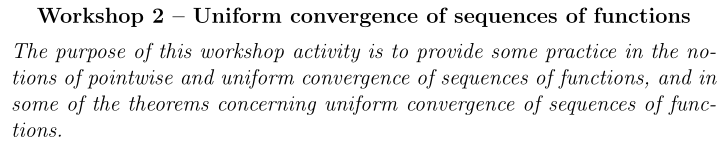
\includegraphics[width=270]{001.png} \\
    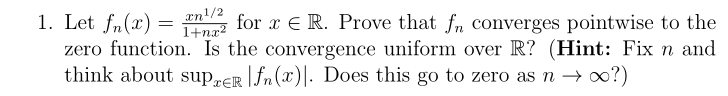
\includegraphics[width=270]{002.png} \\
    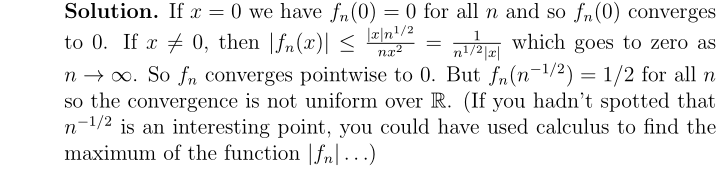
\includegraphics[width=270]{003.png} \\
    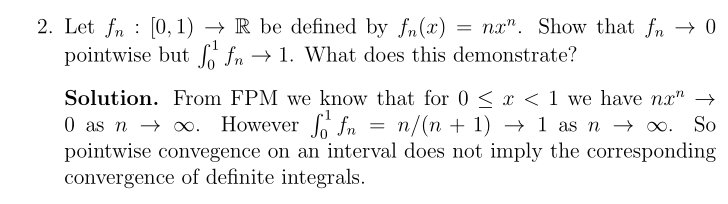
\includegraphics[width=270]{004.png} \\
    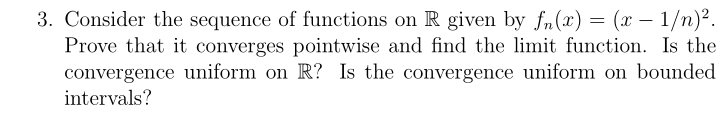
\includegraphics[width=270]{005.png} \\
    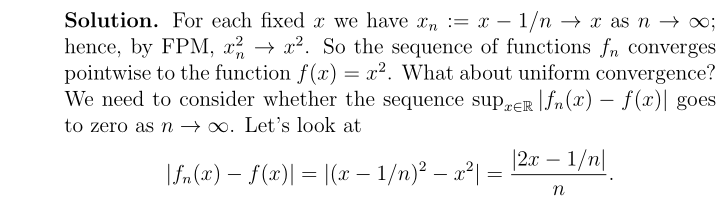
\includegraphics[width=270]{006.png} \\
    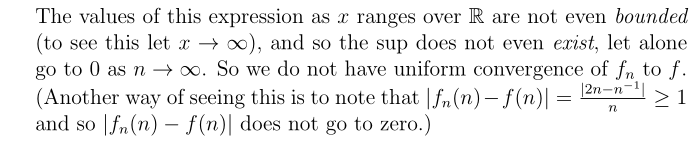
\includegraphics[width=270]{007.png} \\
    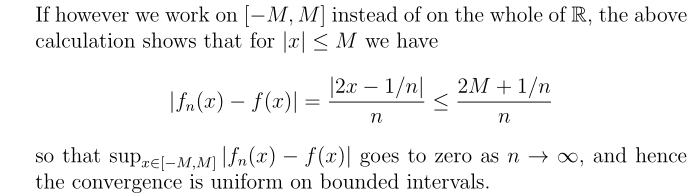
\includegraphics[width=270]{008.png} \\
    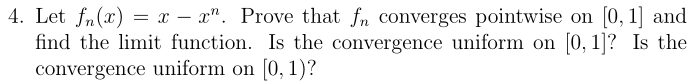
\includegraphics[width=270]{009.png} \\
    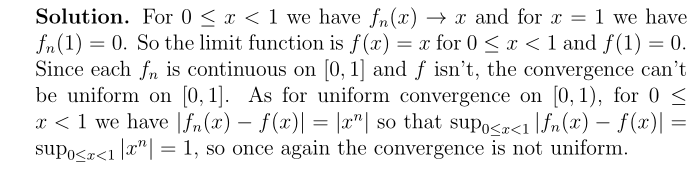
\includegraphics[width=270]{010.png} \\
    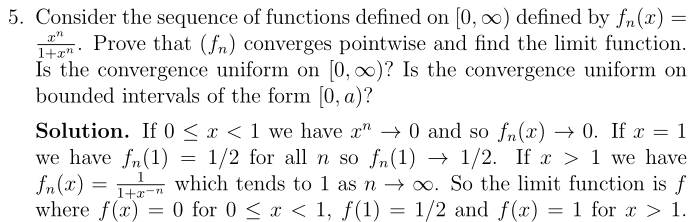
\includegraphics[width=270]{011.png} \\
    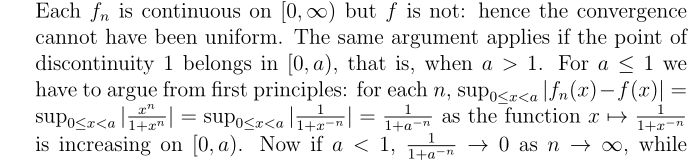
\includegraphics[width=270]{012.png} \\
    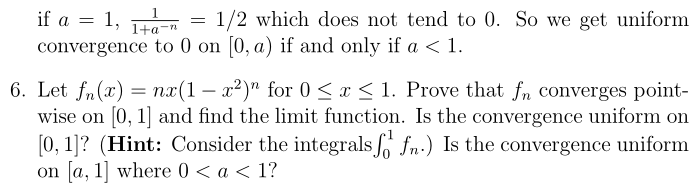
\includegraphics[width=270]{013.png} \\
    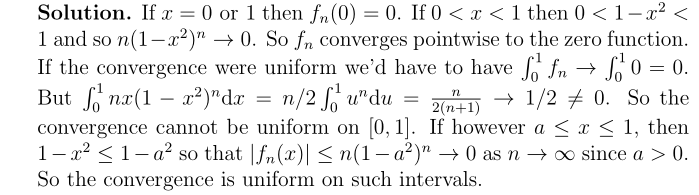
\includegraphics[width=270]{014.png} \\
    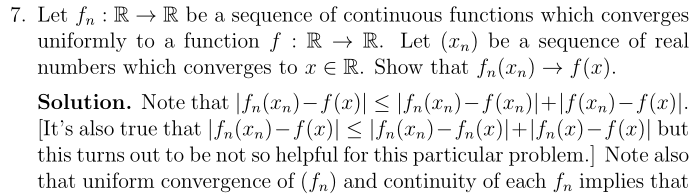
\includegraphics[width=270]{015.png} \\
    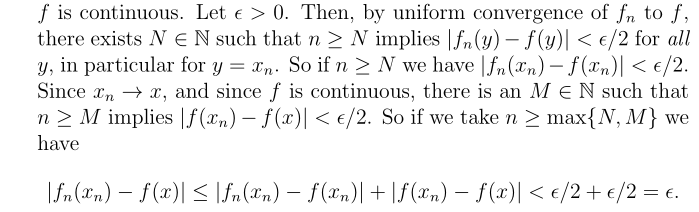
\includegraphics[width=270]{016.png} \\
    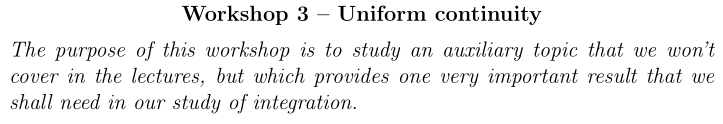
\includegraphics[width=270]{017.png} \\
    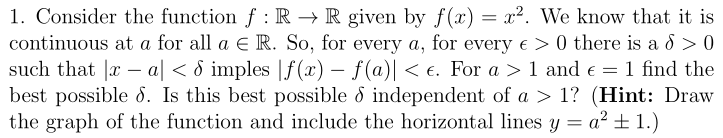
\includegraphics[width=270]{018.png} \\
    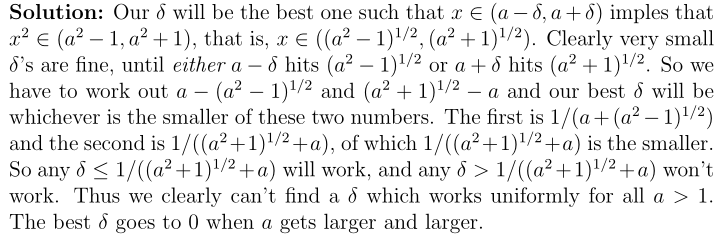
\includegraphics[width=270]{019.png} \\
    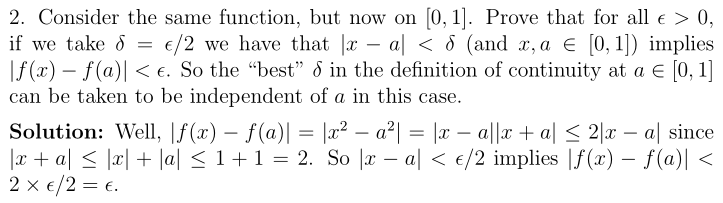
\includegraphics[width=270]{020.png} \\
    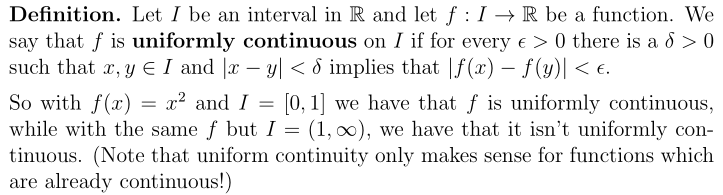
\includegraphics[width=270]{021.png} \\
    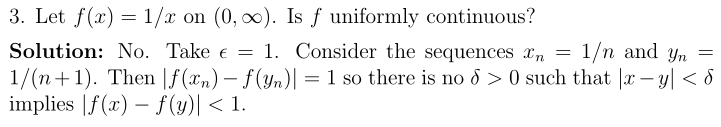
\includegraphics[width=270]{022.png} \\
    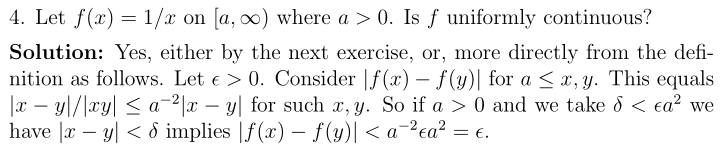
\includegraphics[width=270]{023.png} \\
    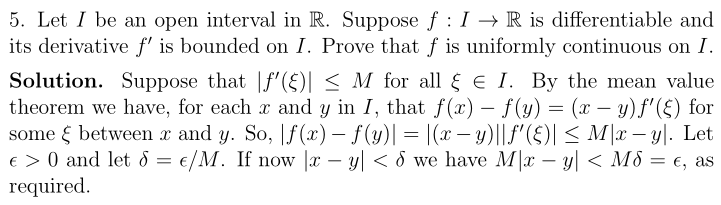
\includegraphics[width=270]{024.png} \\
    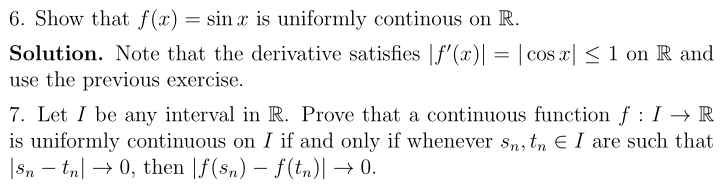
\includegraphics[width=270]{025.png} \\
    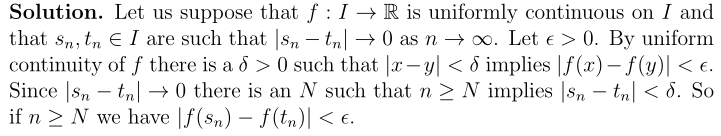
\includegraphics[width=270]{026.png} \\
    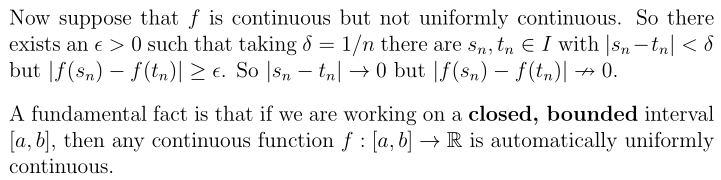
\includegraphics[width=270]{027.png} \\
    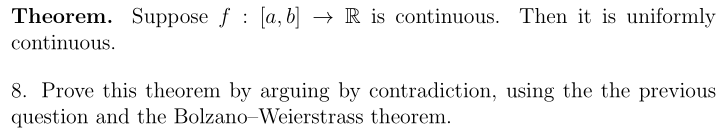
\includegraphics[width=270]{028.png} \\
    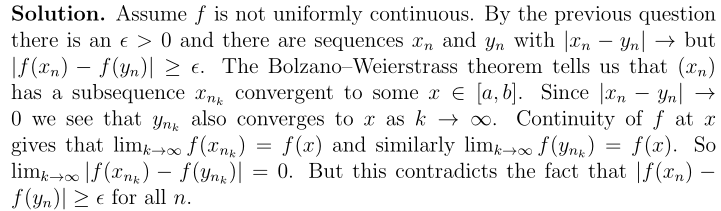
\includegraphics[width=270]{029.png} \\
    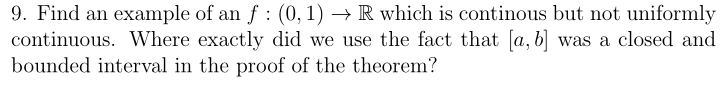
\includegraphics[width=270]{030.png} \\
    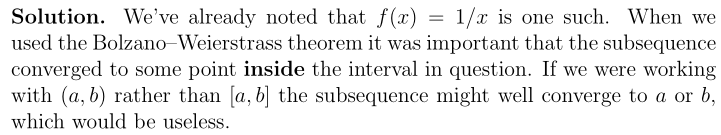
\includegraphics[width=270]{031.png} \\
    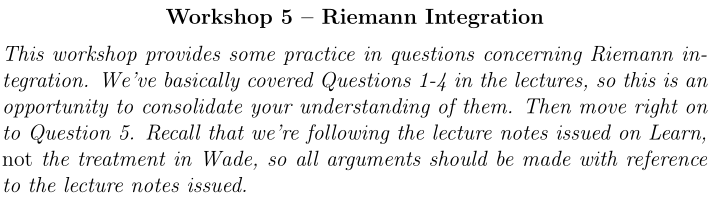
\includegraphics[width=270]{032.png} \\
    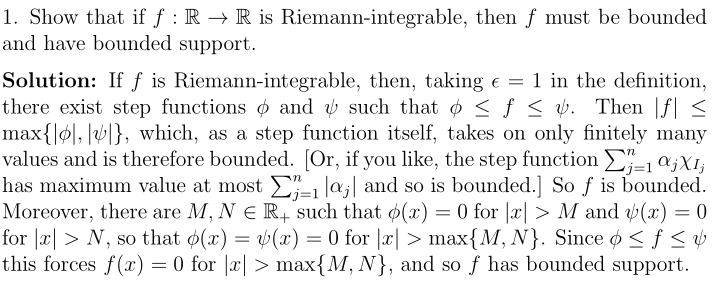
\includegraphics[width=270]{033.png} \\
    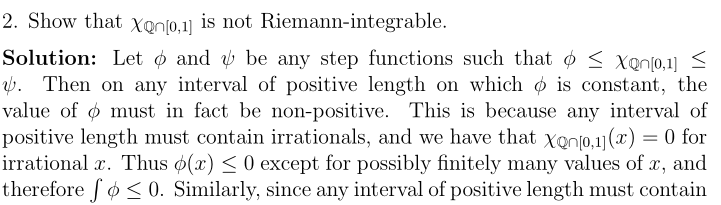
\includegraphics[width=270]{034.png} \\
    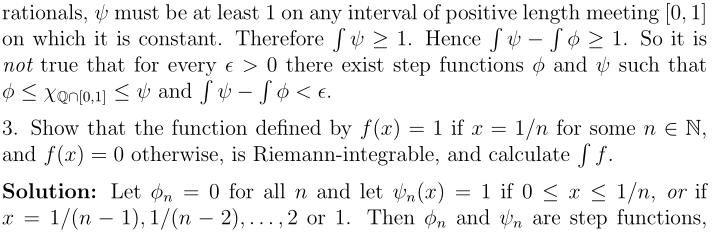
\includegraphics[width=270]{035.png} \\
    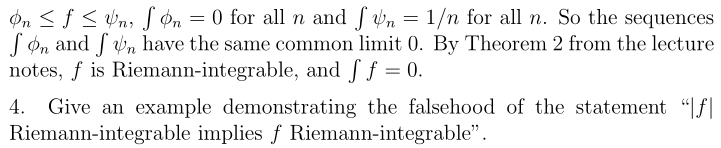
\includegraphics[width=270]{036.png} \\
    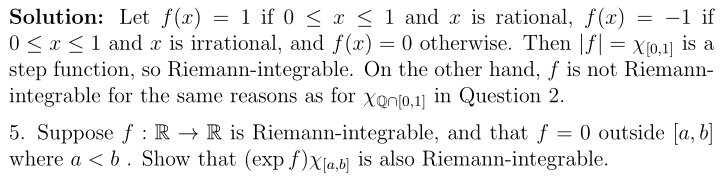
\includegraphics[width=270]{037.png} \\
    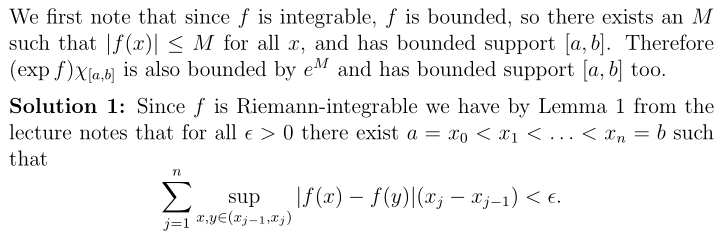
\includegraphics[width=270]{038.png} \\
    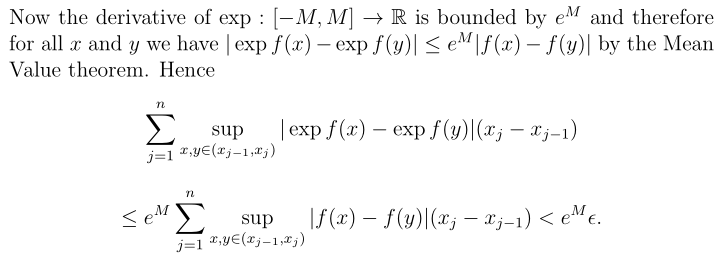
\includegraphics[width=270]{039.png} \\
    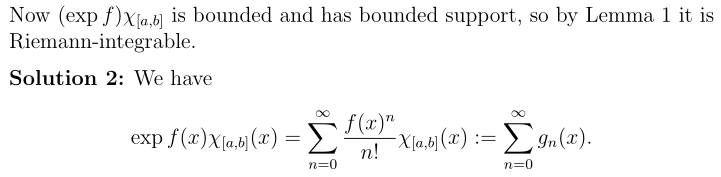
\includegraphics[width=270]{040.png} \\
    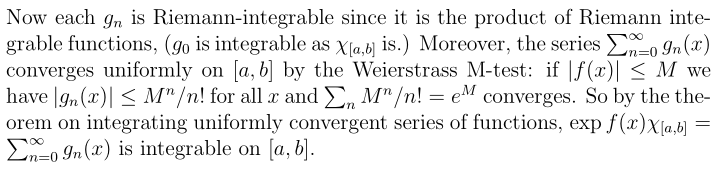
\includegraphics[width=270]{041.png} \\
    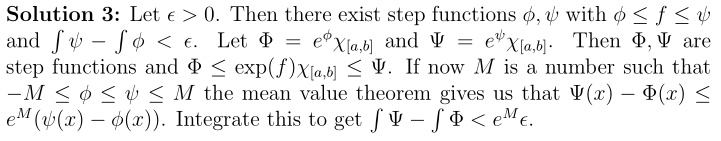
\includegraphics[width=270]{042.png} \\
    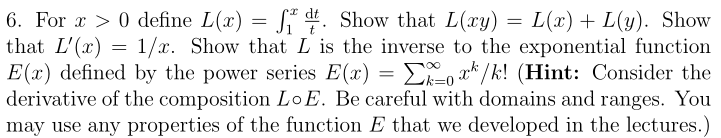
\includegraphics[width=270]{043.png} \\
    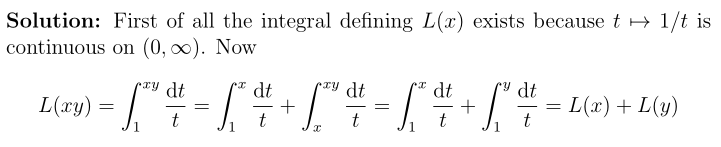
\includegraphics[width=270]{044.png} \\
    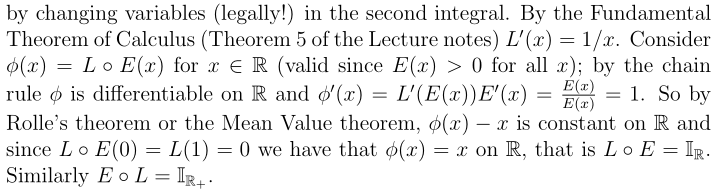
\includegraphics[width=270]{045.png} \\
    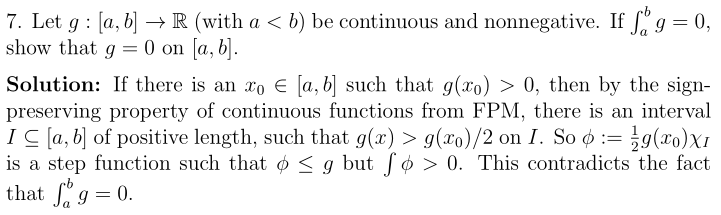
\includegraphics[width=270]{046.png} \\
    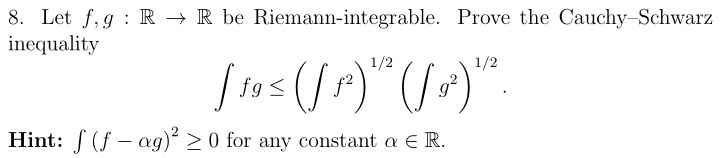
\includegraphics[width=270]{047.png} \\
    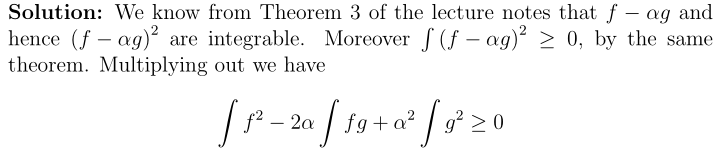
\includegraphics[width=270]{048.png} \\
    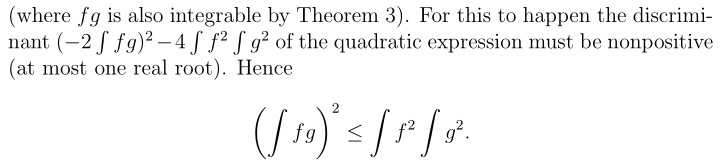
\includegraphics[width=270]{049.png} \\
    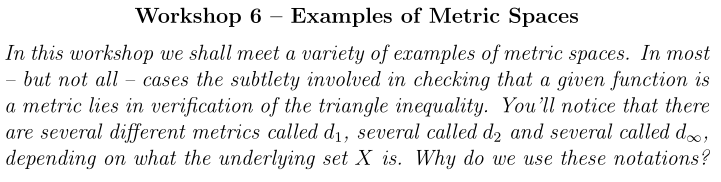
\includegraphics[width=270]{050.png} \\
    \includegraphics[width=270]{051.png} \\
    \includegraphics[width=270]{052.png} \\
    \includegraphics[width=270]{053.png} \\
    \includegraphics[width=270]{054.png} \\
    \includegraphics[width=270]{055.png} \\
    \includegraphics[width=270]{056.png} \\
    \includegraphics[width=270]{057.png} \\
    \includegraphics[width=270]{058.png} \\
    \includegraphics[width=270]{059.png} \\
    \includegraphics[width=270]{060.png} \\
    \includegraphics[width=270]{061.png} \\
    \includegraphics[width=270]{062.png} \\
    \includegraphics[width=270]{063.png} \\
    \includegraphics[width=270]{064.png} \\
    \includegraphics[width=270]{065.png} \\
    \includegraphics[width=270]{066.png} \\
    \includegraphics[width=270]{067.png} \\
    \includegraphics[width=270]{068.png} \\
    \includegraphics[width=270]{069.png} \\
    \includegraphics[width=270]{070.png} \\
    \includegraphics[width=270]{071.png} \\
    \includegraphics[width=270]{072.png} \\
    \includegraphics[width=270]{073.png} \\
    \includegraphics[width=270]{074.png} \\
    \includegraphics[width=270]{075.png} \\
    \includegraphics[width=270]{076.png} \\
    \includegraphics[width=270]{077.png} \\
    \includegraphics[width=270]{078.png} \\
    \includegraphics[width=270]{079.png} \\
    \includegraphics[width=270]{080.png} \\
    \includegraphics[width=270]{081.png} \\
    \includegraphics[width=270]{082.png} \\
    \includegraphics[width=270]{083.png} \\
    \includegraphics[width=270]{084.png} \\
    \includegraphics[width=270]{085.png} \\
    \includegraphics[width=270]{086.png} \\
    \includegraphics[width=270]{087.png} \\
    \includegraphics[width=270]{088.png} \\
    \includegraphics[width=270]{089.png} \\
    \includegraphics[width=270]{090.png} \\
    \includegraphics[width=270]{091.png} \\
    \includegraphics[width=270]{092.png} \\
    \includegraphics[width=270]{093.png} \\
    \includegraphics[width=270]{094.png} \\
    \includegraphics[width=270]{095.png} \\
    \includegraphics[width=270]{096.png} \\
    \includegraphics[width=270]{097.png} \\
    \includegraphics[width=270]{098.png} \\
    \includegraphics[width=270]{099.png} \\
    \includegraphics[width=270]{100.png} \\
    \includegraphics[width=270]{101.png} \\
    \includegraphics[width=270]{102.png} \\
    \includegraphics[width=270]{103.png} \\
    \includegraphics[width=270]{104.png} \\
    \includegraphics[width=270]{105.png} \\
    \includegraphics[width=270]{106.png} \\
    \includegraphics[width=270]{107.png} \\
    \includegraphics[width=270]{108.png} \\
    \includegraphics[width=270]{109.png} \\
    \includegraphics[width=270]{110.png} \\
    \includegraphics[width=270]{111.png} \\
    \includegraphics[width=270]{112.png} \\
    \includegraphics[width=270]{113.png} \\
    \includegraphics[width=270]{114.png} \\
    \includegraphics[width=270]{115.png} \\
    \includegraphics[width=270]{116.png} \\
    \includegraphics[width=270]{117.png} \\
    \includegraphics[width=270]{118.png} \\
    \includegraphics[width=270]{119.png} \\
    \includegraphics[width=270]{120.png} \\
    \includegraphics[width=270]{121.png} \\
    \includegraphics[width=270]{122.png} \\
    \includegraphics[width=270]{123.png} \\
    \includegraphics[width=270]{124.png} \\
    \includegraphics[width=270]{125.png} \\
    \includegraphics[width=270]{126.png} \\
    \includegraphics[width=270]{127.png} \\
    \includegraphics[width=270]{128.png} \\
    \includegraphics[width=270]{129.png} \\
    \includegraphics[width=270]{130.png} \\
    \includegraphics[width=270]{131.png} \\
    \includegraphics[width=270]{132.png} \\
    \includegraphics[width=270]{133.png} \\
    \includegraphics[width=270]{134.png} \\
    \includegraphics[width=270]{135.png} \\
    \includegraphics[width=270]{136.png} \\
    \includegraphics[width=270]{137.png} \\
    \includegraphics[width=270]{138.png} \\
    \includegraphics[width=270]{139.png} \\
    \includegraphics[width=270]{140.png} \\
    \includegraphics[width=270]{141.png} \\
    \includegraphics[width=270]{142.png} \\
    \includegraphics[width=270]{143.png} \\
    \includegraphics[width=270]{144.png} \\
    \includegraphics[width=270]{145.png} \\
    \includegraphics[width=270]{146.png} \\
    \includegraphics[width=270]{147.png} \\
    \includegraphics[width=270]{148.png} \\
    \includegraphics[width=270]{149.png} \\
    \includegraphics[width=270]{150.png} \\
    \includegraphics[width=270]{151.png} \\
    \includegraphics[width=270]{152.png} \\
    \includegraphics[width=270]{153.png} \\
    \includegraphics[width=270]{154.png} \\
    \includegraphics[width=270]{155.png} \\
    \includegraphics[width=270]{156.png} \\
    \includegraphics[width=270]{157.png} \\
    \includegraphics[width=270]{158.png} \\
    \includegraphics[width=270]{159.png} \\
    \includegraphics[width=270]{160.png} \\
    \includegraphics[width=270]{161.png} \\
    \includegraphics[width=270]{162.png} \\
\end{multicols}
\begin{multicols}{3}
    07.02
    \includegraphics[width=250]{07_02.png} \\
    07.03a
    \includegraphics[width=250]{07_03a.png} \\
    07.03b
    \includegraphics[width=250]{07_03b.png} \\
    07.04
    \includegraphics[width=250]{07_04.png} \\
    07.05
    \includegraphics[width=250]{07_05.png} \\
    07.06
    \includegraphics[width=250]{07_06a.png} \\
    \includegraphics[width=250]{07_06b.png} \\
    07.09
    \includegraphics[width=250]{07_09a.png} \\
    \includegraphics[width=250]{07_09b.png} \\
    07.10
    \includegraphics[width=250]{07_10.png} \\
    07.11
    \includegraphics[width=250]{07_11a.png} \\
    \includegraphics[width=250]{07_11b.png} \\
    07.12
    \includegraphics[width=250]{07_12a.png} \\
    \includegraphics[width=250]{07_12b.png} \\
    07.15
    \includegraphics[width=250]{07_15.png} \\
    10.09
    \includegraphics[width=250]{10_09.png} \\
    10.10
    \includegraphics[width=250]{10_10.png} \\
    10.11
    \includegraphics[width=250]{10_11.png} \\
    10.15
    \includegraphics[width=250]{10_15.png} \\
    10.16
    \includegraphics[width=250]{10_16.png} \\
    10.17
    \includegraphics[width=250]{10_17.png} \\
    10.18
    \includegraphics[width=250]{10_18.png} \\
    10.21
    \includegraphics[width=250]{10_21.png} \\
    10.31
    \includegraphics[width=250]{10_31a.png} \\
    \includegraphics[width=250]{10_31b.png} \\
    10.32
    \includegraphics[width=250]{10_32.png} \\
    10.34
    \includegraphics[width=250]{10_34.png} \\
    10.39
    \includegraphics[width=250]{10_39a.png} \\
    \includegraphics[width=250]{10_39b.png} \\
    10.40
    \includegraphics[width=250]{10_40.png} \\
    10.43
    \includegraphics[width=250]{10_43.png} \\
    10.44
    \includegraphics[width=250]{10_44.png} \\
    10.45
    \includegraphics[width=250]{10_45.png} \\
    10.46
    \includegraphics[width=250]{10_46.png} \\
    10.47
    \includegraphics[width=250]{10_47.png} \\
    10.49
    \includegraphics[width=250]{10_49.png} \\
    10.50
    \includegraphics[width=250]{10_50a.png} \\
    \includegraphics[width=250]{10_50b.png} \\
    10.52
    \includegraphics[width=250]{10_52a.png} \\
    \includegraphics[width=250]{10_52b.png} \\
    10.55
    \includegraphics[width=250]{10_55.png} \\
    10.56
    \includegraphics[width=250]{10_56a.png} \\
    \includegraphics[width=250]{10_56b.png} \\
    10.58
    \includegraphics[width=250]{10_58.png} \\
    10.61
    \includegraphics[width=250]{10_61.png} \\
    10.62
    \includegraphics[width=250]{10_62.png} \\
    10.63
    \includegraphics[width=250]{10_63.png} \\
    10.64
    \includegraphics[width=250]{10_64.png} \\
\end{multicols}

\begin{multicols}{2}
    Riemann Prop 1
    \includegraphics[width=400]{R_p1.png} \\
    Riemann Theorem 1
    \includegraphics[width=400]{R_t1a.png} \\
    \includegraphics[width=400]{R_t1b.png} \\
    Riemann Theorem 1
    \includegraphics[width=400]{R_t2.png} \\
    Riemann Lemma 1
    \includegraphics[width=400]{R_l1a.png} \\
    \includegraphics[width=400]{R_l1b.png} \\
    Riemann Theorem 3
    \includegraphics[width=400]{R_t3.png} \\
    Riemann Theorem 4
    \includegraphics[width=400]{R_t4.png} \\
    Riemann Theorem 5
    \includegraphics[width=400]{R_t5.png} \\
    Riemann Theorem 6
    \includegraphics[width=400]{R_t6.png} \\
    Riemann Theorem 7
    \includegraphics[width=400]{R_t7a.png} \\
    \includegraphics[width=400]{R_t7b.png} \\

    Power Theorem 1
    \includegraphics[width=400]{P_t1.png} \\
    Power Theorem 2
    \includegraphics[width=400]{P_t2a.png} \\
    \includegraphics[width=400]{P_t2b.png} \\
    Power Lemma 1
    \includegraphics[width=400]{P_l1.png} \\
    Power Theorem 3
    \includegraphics[width=400]{P_t3.png} \\

    % \textbf{Contraction Mappings}
    Contraction Theorem 1
    \includegraphics[width=400]{B_t1a.png} \\
    \includegraphics[width=400]{B_t1b.png} \\
    % Contraction Theorem 2
    % \includegraphics[width=400]{B_t2a.png} \\
    % \includegraphics[width=400]{B_t2b.png} \\

\end{document}
